\documentclass[12pt,a4paper]{report}
\usepackage[
left=2.5cm, right=4cm, top=2.5cm, bottom=2.5cm]{geometry}
\usepackage{mathtools}
\usepackage{multirow}
\usepackage{setspace}
\usepackage{float}
\usepackage{physics}
\usepackage[table,xcdraw]{xcolor}
\usepackage{mathtools}
\usepackage{amsmath}
\usepackage{gensymb}
\usepackage{caption}
\usepackage{hyperref}
\restylefloat{table}
\setlength{\parindent}{0pt}
\begin{document}
\raggedbottom
\onehalfspacing

\title{Machine Dynamics (MCEN2003) \\  Laboratory Report}
\author{Dicky Larson Gultom \\ 19487537 \\}
\date{\today}
\maketitle

\newpage
\pagenumbering{roman}
\chapter*{Abstract}
\addcontentsline{toc}{chapter}{Abstract}
The purpose of this document is to analyse the experimental data that are provided by the lecturer for all three experiments: mass moment of inertia of a piston, belt friction and epicyclic gear velocity ratio. \\

The first problem this document attempt to solve is to determine the mass moment of inertia of a piston using two commonly used laboratory method to determine the mass moment of inertia of an object; the compound pendulum method and the trifilar suspension method. In addition to determining the mass moment inertia of the piston, this laboratory report also explore which method will gives the most accurate result based on uncertainty. The second problem is to determine the coefficient of friction of a belt using coil rig configuration and vee-belt configuration. Lastly, the last problem is to determine the velocity ratio between the input and the output while locking either the carrier arm, the sun gear and the annulus or ring gear.\\

The results shows that for the first experiment (mass moment of inertia experiment), the trifilar method will yield the most accurate mass moment inertia because it has the lowest final uncertainty with approximately $2\%$ compared to compound pendulum method with $9\%$. For the second experiment, the result shows that the coil rig configuration has a lower coefficient of friction $\mu$ value compared to vee belt configuration. Lastly, the final results for the epicyclic gear experiment show the ratio between the sun gear and the annulus gear when the carrier arm is fixed is 3 to 1, 4 to 1 for the ratio between the sun and the carrier arm when the annulus gear is fixed and lastly 3 to 4 for the ratio between the carrier arm and the annulus gear when the sun gear is fixed. 

\tableofcontents
\listoffigures
\addcontentsline{toc}{chapter}{List of Figures}

\listoftables
\addcontentsline{toc}{chapter}{List of Tables}
\chapter*{Nomenclature.}
\addcontentsline{toc}{chapter}{Nomenclature.}
\section*{Moment of Inertia Experiment.}
\begin{table}[H]
\begin{tabular}{ll}
$m$             & Mass of the object.                                      \\
$T_a$           & Period of oscillation about point A.                     \\
$T_b$           & Period of oscillation about point B.                     \\
$K_c$           & Radius of gyration.                                      \\
$I_c$           & Moment of inertia about its centre of mass.              \\
$\delta I_c$    & The uncertainty of the moment of inertia.                \\
$h$             & The height of the suspension cable.                      \\
$d$             & The diameter of the suspension cable.                    \\
$q_1, q_2, q_3$ & The distance between each suspension cable respectively. \\
$T_{pm}$        & The period of oscillation of the platform and the mass   \\
$T_p$           & The period of oscillation the platform itself.           \\
$g$             & The acceleration due to gravity                          \\
$G$             & The modulus of rigidity of the steel suspension wires.   \\
$M_p$           & Mass of the empty platform.                     
\end{tabular}
\caption*{}
\label{tab:my-table}
\end{table}

\section*{Belt Friction Experiment.}
\begin{table}[H]
\begin{tabular}{ll}
$T_1$                   & Tension on the tight side.                                       \\
$T_2$                   & Tension on the slack side.                                       \\
$\mu$                   & The coefficient of friction.                                     \\
$\mu '$                 & A term that is given by $\mu *\csc\left(\frac{\alpha}{2}\right)$ \\
$\alpha$ & The vee belt angle.                                              \\
$\theta$                & The angle between the slack side and the tight side.            
\end{tabular}
\caption*{}
\label{tab:my-table}
\end{table}

\section*{Epicyclic Gears Experiement.}
\begin{table}[H]
\begin{tabular}{ll}
$T_x$    & The total number of teeth of gear x.                                    \\          
$planet_1$    &  A planet gear that meshes directly with the sun gear.                                 \\
$planet_2$  & A planet gear that meshes directly with the annulus or ring gear. \\   
\end{tabular}
\caption*{}
\label{tab:my-table}
\end{table}
\cleardoublepage

\pagenumbering{arabic}

\section*{1.0 Introduction.}
\addcontentsline{toc}{chapter}{1.0 Introduction.}
The laboratory experiments for this unit are divided into three different experiments where each experiment explores different topic in machine dynamics. The first experiment is about mass moment of inertia of an object, the second experiment is about belt friction around a pulley and the last experiment is about analysing gear speed ratio in planetary gear system. \\

The purpose of this report is to fulfill the aim of each experiment by analysing the experimental results using the formulae that are given in the lecture slides or the laboratory script itself.

\section*{2.0 Mass Moment of Inertia Estimation.}
\addcontentsline{toc}{chapter}{2.0 Mass Moment of Inertia Estimation.}
The aim of this experiment is to explore experimental techniques such as compound pendulum technique and trifilar suspension technique to determine the mass moment of inertia of an object.\\

The analysis below uses the experimental data sets that were published on machine dynamics blackboard. In this data sets, the assumptions are that a digital scale was used to measure the weight of the connecting rod and a standard 60cm ruler was used to measure the length of the connecting rod. In addition to those two apparatuses, a stopwatch that can measure 1/100 seconds was also used to calculate the oscillation period.  \\

\subsection*{2.1 Analysis of Compound Pendulum Method.}
\addcontentsline{toc}{section}{2.1 Analysis of Compound Pendulum Method.}
The two constants for this method of experiment are the mass of the connecting rod which is weighted to be 2.65 kg $\pm$ 0.1 kg and the length of the connecting rod which has a length of 0.33 m $\pm$ 0.001 m. \\

The two trials experimental results are shown on the table below where the first trial will the period of natural oscillations at point A and the second trials will the period of natural oscillations at point B. In addition that, each trials are repeated thrice as suggested by the laboratory guide. The experimental setup is shown on the figure below:\\
\begin{figure}[H]
\centering
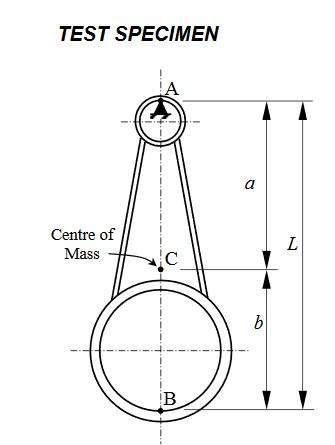
\includegraphics[width=0.5\textwidth]{chapters/lab1/m1}
\caption{Experimental setup for compound pendulum method.}
\label{fig:mesh2}
\end{figure}

\begin{table}[h!]
\begin{tabular}[b]{ | c | c | c | c | }
\hline
 & $T_{A1}$ & $T_{A2}$ & $T_{A3}$\\
\hline
\multirow{5}{10em}{Period (Seconds)} & 53.06 $\pm$ 0.01 & 52.97 $\pm$ 0.01  & 53.06 $\pm$ 0.01 \\
& 52.75 $\pm$ 0.01 & 52.93 $\pm$ 0.01 & 52.97 $\pm$ 0.01 \\
&52.91 $\pm$ 0.01 & 53.05 $\pm$ 0.01 & 53.06 $\pm$ 0.01 \\
& 53.03 $\pm$ 0.01 & 52.97 $\pm$ 0.01 & 53.19 $\pm$ 0.01 \\ 
& 53.11 $\pm$ 0.01 & 53.18 $\pm$ 0.01 & 53.13 $\pm$ 0.01 \\
\hline
\end{tabular}
\caption{Natural oscillations period about point A.}
\label{table:1}
\end{table}

\begin{table}[H]
\begin{tabular}[b]{ | c | c | c | c |}
\hline
& $T_{B1}$ & $T_{B2}$ & $T_{B3}$\\
\hline
\multirow{5}{10em}{Period (Seconds)} & 47.57 $\pm$ 0.01 & 47.63 $\pm$ 0.01 & 47.67 $\pm$ 0.01 \\
& 47.66 $\pm$ 0.01 & 47.44 $\pm$ 0.01 & 47.59 $\pm$ 0.01 \\
&47.72 $\pm$ 0.01 & 47.38 $\pm$ 0.01 & 47.69 $\pm$ 0.01 \\
&47.59 $\pm$ 0.01 & 447.44 $\pm$ 0.01 & 48.91 $\pm$ 0.01 \\
&48.32 $\pm$ 0.01 & 47.56 $\pm$ 0.01 & 47.53 $\pm$ 0.01 \\
\hline
\end{tabular}
\caption{Natural oscillations period about point B.}
\label{table:2}
\end{table}



\hspace{0pt}Since the technique used to determine the moment of inertia is using pendulum-like technique, hence the equation of mass moment of inertia about the principal axis through centre of mass $C$ and perpendicular to the plane of the connecting rod $I_c$ can be derived from simple pendulum equation and its derivation is shown in the laboratory manuals. The equation of mass-moment of inertia is as shown below: 
\begin{equation}\label{eq:1}
 I_c = m \times {k_c}^2 
\end{equation}
Where $m$ is the mass of the connecting rod in kilograms and ${k_c}^2$ is given by:
\begin{equation}\label{eq:2}
k_c^2 = 0.2483 \times b \times T_B^2 - b^2
\end{equation}
Substituting $k_c^2$ from equation \ref{eq:2} into equation \ref{eq:1}, therefore the equation for mass moment of inertia $I_c$ becomes:
\begin{equation}
I_c = m \times (0.2483 \times b \times T_B^2 - b^2)
\end{equation}
Where $b$ is equivalent to, \begin{equation} b = \frac{L}{1 + \frac{L- 0.2483 \times T_B^2}{L - 0.2483 \times T_A^2}}\end{equation}
To find the value both $T_A$ and $T_B$, we can use the equation given in the laboratory script. However, we firstly need to calculate the average time taken for 50 complete oscillations of each trial for both at point A and point B. The average time taken for both point A and B are shown on the table below: \\
\begin{table}[h]
\begin{center}
\begin{tabular}{c|c|c|c|}
\cline{2-4}
 & $T_{A1}$ & $T_{A2}$ & $T_{A3}$ \\ \hline
\multicolumn{1}{|c|}{$T_{ave}$(Seconds)} & {\color[HTML]{000000} 52.972 $\pm$ 0.01} & {\color[HTML]{000000} 53.020 $\pm$ 0.01} & {\color[HTML]{000000} 53.082 $\pm$ 0.09} \\ \hline
\end{tabular}
\caption{Average natural oscillations period in seconds for each trial at point A.}
\label{tab:3}
\end{center}
\end{table}

\begin{table}[h]
\begin{center}
\begin{tabular}{c|c|c|c|}
\cline{2-4}
 & $T_{B1}$ & $T_{B2}$ & $T_{B3}$ \\ \hline
\multicolumn{1}{|c|}{$T_{ave}$(Seconds)} & {\color[HTML]{000000} 47.772 $\pm$ 0.01} & {\color[HTML]{000000} 47.49 $\pm$ 0.01} & {\color[HTML]{000000} 47.878 $\pm$ 0.01} \\ \hline
\end{tabular}
\caption{Average natural oscillations period in seconds for each trial at point B.}
\label{tab:4}
\end{center}
\end{table}
Using the values above, therefore the period about a point can be calculated by summing the average time taken for 50 complete oscillations and then divide by 150. The period for oscillating at point A and B and its uncertainty are shown below:
\[T_A= \frac{52.972 + 53.020 + 53.082}{150} = 1.06 \pm 0.01 seconds.\]
\[T_B= \frac{47.772 + 47.49 + 47.878}{150} =  0.95\pm 0.01 seconds.\]

By substituting the value of $T_A$ and $T_B$ to into equation 4, then the value of b is calculated to be:
\[b = \frac{0.33}{1 + \frac{0.33 - 0.2483 * 0.95^2}{0.33 - 0.2483 * 1.06^2}}\]
\[b = 0.107\]
In addition to that, using the technique as prescribed in the error/uncertainty analysis document on Blackboard then the uncertainty of the equation 4 is given by:
\begin{align}
\delta b &= \pm \abs{\left(\dfrac{2L^2-2\left(T_B^2+T_A^2\right)zL+T_A^2\left(T_B^2+T_A^2\right)z^2}{\left(2L-\left(T_B^2+T_A^2\right)z\right)^2}\right)\delta L} \notag \\
&\qquad + \abs{\left(\dfrac{2Lz(T_B^2z-L)T_A}{(zT_A^2+T_B^2z-2L)^2}\right)\delta T_A} \notag \\ 
&\qquad + \abs{\left(-\dfrac{2Lz\left(T_A^2z-L\right)T_B}{\left(zT_B^2+T_A^2z-2L\right)^2}\right)\delta T_B} \notag
\end{align}

Where $z$ is equal to 0.2483. Substituting the value for $z$, $T_A$, $T_B$ and $L$ back into the equation above, then the equation becomes: \\
\begin{align}
\delta b &= \pm \abs{\left(\dfrac{2*0.33^2-2\left(0.95^2+1.06^2\right)*0.2483*0.33+1.06^2\left(0.95^2+1.06^2\right)*0.2483^2}{\left(2*0.33-\left(0.95^2+1.06^2\right)*0.2483\right)^2}\right)(0.001)} \notag \\
&\qquad + \abs{\left(\dfrac{2*0.33*0.2483(0.95^2*0.2483-0.33)1.06}{(0.2483*1.06^2+0.95^2*0.2483-2*0.33)^2}\right)(0.01)} \notag \\ 
&\qquad + \abs{\left(-\dfrac{2*0.33*0.2483\left(1.06^2*0.2483-0.33\right)0.95}{\left(0.2483*0.95^2+1.06^2*0.2483-2*0.33\right)^2}\right)(0.01)} \notag \\
&=  0.0010608154258371118 + 0.007471491405688022 + 0.003225131996229406 \notag \\
&= 0.012 \notag \\
b &= 0.107 \pm 0.012 \notag
\end{align}

Substituting the value of $b$ into equation 2 and applying the same technique to calculate uncertainty, then the mass moment of inertia of the object and its uncertainty values calculated to be:
\begin{align}
I_c &= 2.65(0.2483 * 0.107 * 0.95^2 - 0.0.7^2) \notag \\
&= 0.033 kg.m^2 \notag \\
\delta I_c &= \abs{\left(0.2483*b*T_B^2-b^2\right)(\delta m)} + \abs{\left(m(0.2483*T_B^2-2b)\right)(\delta b)} \notag \\
&\qquad + \abs{(2*0.2483*b*m*T_B)(\delta T_B)} \notag \\
&= \abs{\left(0.2483*0.107*0.95^2-0.107^2\right)(0.1)} + \abs{\left(2.65(0.2483*0.95^2-2*0.107)\right)(0.012)} \notag \\
&\qquad + \abs{(2*0.2483*0.107*2.65*0.95)(0.01)} \notag \\
&= 0.003 \notag \\
I_c &= 0.033 \pm 0.003 kg.m^2 \notag 
\end{align}

\subsection*{2.2 Analysis of Trifilar Suspension Method.}
For this method of experiment, the assumption is the apparatus are still the same apparatus as previous experiment i.e. ruler to measure length, stopwatch to measure time and digital scale to determine the mass. In addition to that, slide calliper is also used to measure the diameter of the haging cable. In this experiment the constants are:
\begin{itemize}
\item Height of the cable $=$ 1.87 $\pm$ 0.1 m
\item Diameter of the cable $=$ 0.00132 $\pm$ 0.0001 m
\item $q_1$ $=$ 0.1313 $\pm$ 0.001 m
\item $q_2$ $=$ 0.1312 $\pm$ 0.001 m
\item $q_3$ $=$ 0.1314 $\pm$ 0.001 m
\item Mass of the empty platform $=$ 1.997 $\pm$ 0.1 kg.
\end{itemize}
The experimental setup for this experiment is shown on the figures below:
\begin{figure}[H]
\centering
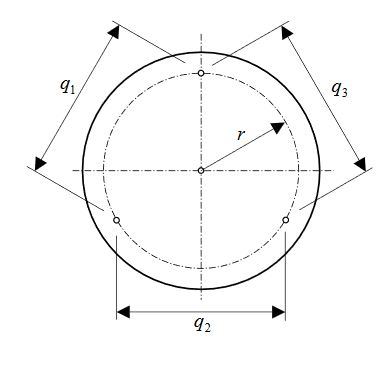
\includegraphics[width=0.5\textwidth]{chapters/lab1/m2topdown}
\caption{Top down view experimental setup for trifilar suspension method.}
\label{fig:mesh2}
\end{figure}
\begin{figure}[H]
\centering
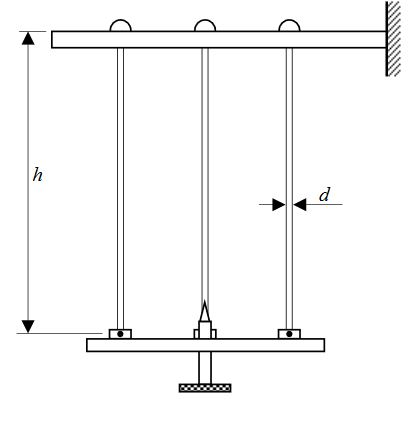
\includegraphics[width=0.5\textwidth]{chapters/lab1/m2}
\caption{Experimental setup for trifilar suspension method.}
\label{fig:mesh2}
\end{figure}

The three readings for the time taken for 40 complete oscillations of the platform carrying the object mass $m$ with oscillations amplitude of approximately 5$^\circ$ and the average period are shown on the table below:
\begin{table}[h!]
\begin{center}
\begin{tabular}{c|c|c|c|}
\cline{2-4}
 &
  \multicolumn{3}{c|}{Trial with Connecting Rod} \\ \cline{2-4} 
 &
  1 &
  2 &
  3 \\ \hline
\multicolumn{1}{|c|}{\multirow{5}{*}{Time (Seconds)}} &
  128.03±0.01 &
  127.94±0.01 &
  \begin{tabular}[c]{@{}c@{}}128.18\\ ±0.01\end{tabular} \\ \cline{2-4} 
\multicolumn{1}{|c|}{} &
  127.87±0.01 &
  \begin{tabular}[c]{@{}c@{}}128.03\\ ±0.01\end{tabular} &
  \begin{tabular}[c]{@{}c@{}}128.25\\ ±0.01\end{tabular} \\ \cline{2-4} 
\multicolumn{1}{|c|}{} &
  \begin{tabular}[c]{@{}c@{}}128.31\\ ±0.01\end{tabular} &
  \begin{tabular}[c]{@{}c@{}}128.12\\ ±0.01\end{tabular} &
  \begin{tabular}[c]{@{}c@{}}128.21\\ ±0.01\end{tabular} \\ \cline{2-4} 
\multicolumn{1}{|c|}{} &
  \begin{tabular}[c]{@{}c@{}}128.06\\ ±0.01\end{tabular} &
  \begin{tabular}[c]{@{}c@{}}128.06\\ ±0.01\end{tabular} &
  \begin{tabular}[c]{@{}c@{}}128.38\\ ±0.01\end{tabular} \\ \cline{2-4} 
\multicolumn{1}{|c|}{} &
  \begin{tabular}[c]{@{}c@{}}128.16\\ ±0.01\end{tabular} &
  \begin{tabular}[c]{@{}c@{}}128.07\\ ±0.01\end{tabular} &
  \begin{tabular}[c]{@{}c@{}}128.28\\ ±0.01\end{tabular} \\ \hline
\multicolumn{1}{|l|}{Average} &
  \begin{tabular}[c]{@{}c@{}}128.086\\ ±0.01\end{tabular} &
  \begin{tabular}[c]{@{}c@{}}128.044\\ ±0.01\end{tabular} &
  \begin{tabular}[c]{@{}c@{}}128.26\\ ±0.01\end{tabular} \\ \hline
\end{tabular}
\caption{The time taken for the loaded platform to complete 40 oscillations.}
\label{tab:5}
\end{center}
\end{table}

\begin{table}[h!]
\begin{center}
\begin{tabular}{c|c|c|c|}
\cline{2-4}
 &
  \multicolumn{3}{c|}{Trial with Connecting Rod} \\ \cline{2-4} 
 &
  1 &
  2 &
  3 \\ \hline
\multicolumn{1}{|c|}{\multirow{5}{*}{Time (Seconds)}} &
  85.14±0.01 &
  84.93±0.01 &
  \begin{tabular}[c]{@{}c@{}}84.53\\ ±0.01\end{tabular} \\ \cline{2-4} 
\multicolumn{1}{|c|}{} &
  85.17±0.01 &
  \begin{tabular}[c]{@{}c@{}}84.78\\ ±0.01\end{tabular} &
  \begin{tabular}[c]{@{}c@{}}84.72\\ ±0.01\end{tabular} \\ \cline{2-4} 
\multicolumn{1}{|c|}{} &
  \begin{tabular}[c]{@{}c@{}}85.07\\ ±0.01\end{tabular} &
  \begin{tabular}[c]{@{}c@{}}84.72\\ ±0.01\end{tabular} &
  \begin{tabular}[c]{@{}c@{}}84.66\\ ±0.01\end{tabular} \\ \cline{2-4} 
\multicolumn{1}{|c|}{} &
  \begin{tabular}[c]{@{}c@{}}85.13\\ ±0.01\end{tabular} &
  \begin{tabular}[c]{@{}c@{}}84.75\\ ±0.01\end{tabular} &
  \begin{tabular}[c]{@{}c@{}}84.54\\ ±0.01\end{tabular} \\ \cline{2-4} 
\multicolumn{1}{|c|}{} &
  \begin{tabular}[c]{@{}c@{}}85.03\\ ±0.01\end{tabular} &
  \begin{tabular}[c]{@{}c@{}}84.65\\ ±0.01\end{tabular} &
  \begin{tabular}[c]{@{}c@{}}84.51\\ ±0.01\end{tabular} \\ \hline
\multicolumn{1}{|l|}{Average} &
  \begin{tabular}[c]{@{}c@{}}85.108\\ ±0.01\end{tabular} &
  \begin{tabular}[c]{@{}c@{}}84.766\\ ±0.01\end{tabular} &
  \begin{tabular}[c]{@{}c@{}}84.592\\ ±0.01\end{tabular} \\ \hline
\end{tabular}
\caption{The time taken for the empty platform to complete 40 oscillations.}
\label{tab:6}
\end{center}
\end{table}

Using the formulae given in the laboratory script to find the time period of oscillation, then the time period for both loaded and empty platform to 3 significant figures calculated to be:
\begin{align}
T_{pm} &= \frac{T_{pm1} + T_{pm2} + T_{pm3}}{120} \notag \\
&= \frac{128.086 + 128.044 + 128.26}{120} \notag \\
&= 3.20 \pm 0.01 seconds \notag \\
T_p  &= \frac{T_{p1} + T_{p2} + T_{p3}}{120} \notag \\
&= \frac{85.108 + 84.766 + 84.592}{120} \notag \\
&= 2.12  \pm 0.01 seconds\notag
\end{align}

The derivation to determine the mass moment of inertia $I$ of an object has been done for us in the laboratory script and the equation $I$ is as shown below:
\begin{equation}
I = \frac{gr^2}{4\pi^2h}\left[T_{pm}^2\left(m_p + m\right) - T_p^2m_p\right] + \frac{3Gd^4}{128\pi h}\left(T_{pm}^2-T_p^2\right)
\end{equation}

Where $g$ is the acceleration due to gravity, $G$ the modulus of rigidity of the steel suspension wires, $m_p$ mass of the empty platform, $m$ is the mass of the object, $h$ is the height of the cable, $T_{pm}$ is the period of the loaded platform, $T_p$ is the period of the empty platform and $r^2$ is given by $\frac{\left(q_1 + q_2+ q_3\right)^2}{27}$. To calculate the mass-moment of inertia of the object, we firstly need to calculate the value of $r^2$:
\begin{align}
r^2 &= \frac{(0.1313 + 0.1312 + 0.1314)^2}{27} \notag \\
&= 0.005746563 \notag \\
\delta r^2 &= \frac{2*(q_1 + q_2 + q_3)}{27}(\delta (q_1 + q_2 + q_3)) \notag \\
&=\frac{2*(0.1313+0.1312+0.1314)}{27}(\delta (0.003)) \notag \\
&= 8.75 \times 10^{-5} \notag \\
r^2 &= 0.005746563 \pm 8.75 \times 10^{-5} m^2 \notag
\end{align}
Substituting the value $r^2$ above into equation 5 along with other values that are required to calculate mass-moment of inertia, then the mass-moment of inertia and its uncertainty values are calculated to be:
\begin{align}
I &= \frac{0.005746563*9.794}{4*\pi^2*1.87}\left[3.202325^2\left(1.997 + 2.65\right) - 2.120255^2*1.997\right] \notag \\
&\qquad+ \frac{3*80 \times 10^9*0.00132^4}{128*\pi*1.87}\left(3.20325^2-2.12055^2\right) \notag \\
I &= 0.035 kg.m^2 \notag \\
\delta I &= \pm \abs{\left(\dfrac{3\left(T_{pm}^2-T_p^2\right)Gd^3}{32{\pi^2}h}\right)(\delta d)} \notag \\
&\qquad + \abs{\dfrac{\left(T_{pm}^2\left(m_p+m\right)-T_p^2m_p\right)r^2}{4{\pi^2}h}(\delta g)} \notag \\
&\qquad + \abs{\left(-\dfrac{3d^4\left(T_{pm}^2-T_p^2\right)G}{128{\pi}h^2}-\dfrac{g\left(T_{pm}^2\left(m_p+m\right)-T_p^2m_p\right)r^2}{4{\pi^2}h^2}\right)(\delta h) } \notag \\
&\qquad + \abs{\left(\dfrac{gT_{pm}^2r^2}{4{\pi^2}h}\right)(\delta m)} +  \abs{\dfrac{3d^4GT_{pm}}{64{\pi}h}+\dfrac{g\left(m_p+m\right)r^2T_{pm}}{2{\pi}^2h}(\delta T_{pm})}\notag \\
&\qquad + \abs{\left(-\dfrac{\left(3{\pi}d^4G+32gm_pr^2\right)T_p}{64{\pi^2}h}\right)(\delta T_p)} + \abs{\left(\dfrac{g\left(T_{pm}^2-T_p^2\right)r^2}{4{\pi^2}h}\right)(\delta m_p)} \notag \\
&\qquad + \abs{\left(\dfrac{g\left(T_{pm}^2\left(m_p+m\right)-T_p^2m_p\right)r}{2{\pi^2}h}\right)(\delta r)} \notag \\
\delta I &= 6.60\times10^{-4} \notag \\
I &= 0.035 \pm 6.60\times10^{-4} kg.m^2 \notag
\end{align}
\addcontentsline{toc}{section}{2.2 Analysis of Trifilar Suspension Method.}

\subsection*{2.3 Discussion.}
\addcontentsline{toc}{section}{2.2 Discussion.}
The primary source of uncertainty for both experiments majorly comes from systematic errors such as human reaction, inaccurate apparatus calibration and incorrect measurement reading because these systematic errors cannot be eliminated and corrected with repeated experiment rerun. On the other hand, the effect of random errors in these experiments are negligible because these unlike systematic errors, these errors can be quickly eliminated by taking multiple readings where in this case to oscillate the object three times. In addition to systematic errors above, a non-symmetrical axis between the object's centre of mass and the suspension will cause inaccurate natural oscillation time period for the second experiment.\\

The uncertainty for the first experiment is approximately $9.1\%$ where as for the second experiment, the uncertainty is much lower uncertainty compare to the uncertainty of the first experiment with $1.9\%$. This shows that the moment of inertia calculated using the trifilar method is more accurate compare to the compound pendulum method in terms of uncertainty calculation. On the down side, the trifilar suspension experiment method is more difficult to set up and to carry because the object's centre of mass must be on a symmetry axis of the suspension in order to get an accurate final result whereas the compound pendulum method is much more easier to set up and carry. \\

The trifilar suspension method could be useful if the object's centre of mass is exactly at half the length of the object or at least the location of centre of mass is known and the surface of the object is flat. This condition will make it easier to put the object symmetrically to the suspension axis which at the end will yield more accurate moment of inertia where as in compound pendulum method, we do not need to worry about the object centre of mass. On the other hand, compound pendulum method could be useful if the oscillation amplitude is small because the equation become less valid as the oscillation amplitude increases therefore could affect the final calculation result. 

\section*{3.0 Belt Friction.}
\addcontentsline{toc}{chapter}{3.0 Belt Friction.}
The objective of this experiment is to use limiting belt friction equation given in the laboratory script to find the coefficient of friction $\mu$ of two types of belt-pulley configuration; coil friction belt configuration and vee belt configuration. The configuration used for both belt experiments is shown in the schematic below: \\
\begin{figure}[H]
\centering
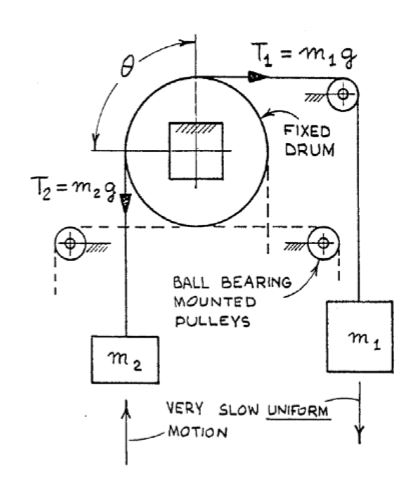
\includegraphics[width=0.5\textwidth]{chapters/lab2/setup}
\caption{Belt configuration.}
\label{fig:mesh1}
\end{figure}
Where $m_2$ is the slack tension side, $m_1$ is the tight tension side and $\theta$ is the angle of lap. Angle of lap is defined as the angle it makes between the slack tension side and the tight tension side. The configuration for the lap angle is shown on the figure below:
\begin{figure}[h!]
\centering
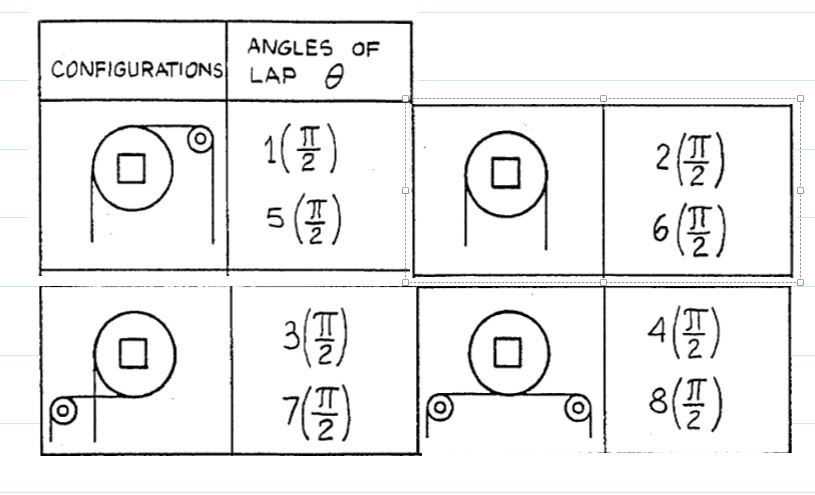
\includegraphics[width=0.7\textwidth]{chapters/lab2/angle}
\caption{Belt lap angle configuration.}
\label{fig:mesh2}
\end{figure}

The limiting belt friction relationship equation is given by:
\begin{equation}
\frac{T_1}{T_2} = e^{\mu'\theta}
\end{equation}
Where $\mu'$ is defined as:
\begin{equation}
\mu' = \mu*\csc\left(\frac{\alpha}{2}\right)
\end{equation}
Where $\alpha$ is the lap angle of the belt in the general configuration.

\subsection*{3.1 Analysis of Coil Friction Experiment.}
\addcontentsline{toc}{section}{3.1 Analysis of Coil Friction Experiment.}

In this part of experiment, coil friction rig configuration is used and it will be used to calculate the coefficient of friction by varying the angle of lap. In addition to that, the slack tension is constant with 0.9 kg of mass and we keep increasing the load on the tight side until the coil belt starts to slip. The measurement experiment reading are shown on the table below:\\
\begin{table}[H]
\begin{center}
\begin{tabular}{|c|c|c|}
\hline
\begin{tabular}[c]{@{}c@{}}Angle \\ \\ (Radian)\end{tabular} & $M_2$ (kg) & $M_1$(kg)   \\ \hline
$\pi$/2                                                          & 0.9$\pm$0.1 & 1.27$\pm$0.1 \\ \hline
3$\pi$/2                                                         & 0.9$\pm$0.1 & 1.88$\pm$0.1 \\ \hline
4$\pi$/2                                                         & 0.9$\pm$0.1 & 2.8$\pm$0.1 \\ \hline
5$\pi$/2                                                         & 0.9$\pm$0.1 & 2.99$\pm$0.1 \\ \hline
6$\pi$/2                                                         & 0.9$\pm$0.1 & 3.44$\pm$0.1 \\ \hline
8$\pi$/2                                                         & 0.9$\pm$0.1 & 6.71$\pm$0.1 \\ \hline
\end{tabular}
\caption{Coil friction experiment results.}
\label{tab: 7}
\end{center}
\end{table}

According to the laboratory script, the ratio between natural logarithm of the tension side $\ln(T_1)$ and the natural logarithm of the slack side $\ln(T_2)$ is constant and it is equal to the product of the lap angle $\theta$ and the coefficient of friction $\mu$. Therefore, it is a linear relationship between tension side $\ln(T_1)$ and  slack side $\ln(T_2)$ and the linear equation is:
\begin{equation}
\ln(T_1) = \mu\theta + \ln(T_2)
\end{equation}
The tension force on each side is equal to the weight force $F_g$ and it is given by $m*g$ where $m$ is the mass of the object and $g$ is the acceleration due to gravity. Since we conduct this experiment on the same location as the moment of inertia experiment, then we can use the same value for the acceleration due to gravity. In addition to that, the uncertainty to tension force of is given by:
\begin{align}
\delta T&=\pm \abs{\left(g\right)(\delta m)} + \abs{\left(m\right)(\delta g)} \notag
\end{align}
The tension for both the slack side and the tight side are given on the table below:
\begin{table}[H]
\begin{center}
\begin{tabular}{|c|c|c|}
\hline
\begin{tabular}[c]{@{}c@{}}Angle \\ (Radian)\end{tabular} & $T_2$ (N)   & $T_1$(N)      \\ \hline
$\pi$/2                                                          & 8.81$\pm$0.98 & 12.44$\pm$0.98  \\ \hline
3$\pi$/2                                                         & 8.81$\pm$0.98 & 18.41$\pm$0.981 \\ \hline
4$\pi$/2                                                         & 8.81$\pm$0.98 & 27.4$\pm$0.982  \\ \hline
5$\pi$/2                                                         & 8.81$\pm$0.98 & 29.28$\pm$0.982 \\ \hline
6$\pi$/2                                                         & 8.81$\pm$0.98 & 33.69$\pm$0.983 \\ \hline
8$\pi$/2                                                         & 8.81$\pm$0.98 & 65.72$\pm$0.986 \\ \hline
\end{tabular}
\caption{Coil tension.}
\label{tab: 8}
\end{center}
\end{table}

Taking the natural logarithm for both $T_2$ and $T_1$, then:
\begin{table}[H]
\begin{center}
\begin{tabular}{|c|c|c|}
\hline
\begin{tabular}[c]{@{}c@{}}Angle \\ (Radian)\end{tabular} & $\ln(T_2)$   & $\ln(T_1)$      \\ \hline
$\pi$/2                                                          & 2.78$\pm$-0.02 & 2.52$\pm$-0.02  \\ \hline
3$\pi$/2                                                         & 2.78$\pm$-0.02 & 2.91$\pm$-0.019 \\ \hline
4$\pi$/2                                                         & 2.78$\pm$-0.02 & 3.31$\pm$-0.018  \\ \hline
5$\pi$/2                                                         & 2.78$\pm$-0.02 & 3.38$\pm$-0.0182 \\ \hline
6$\pi$/2                                                         & 2.78$\pm$-0.02 & 3.52$\pm$-0.0171 \\ \hline
8$\pi$/2                                                         & 2.78$\pm$-0.02 & 4.19$\pm$-0.0141\\ \hline
\end{tabular}
\caption{Natural logarithmic of the coil tension.}
\label{tab: 9}
\end{center}
\end{table}

Plotting the equilibrium values of $\ln(T_1)$ versus $\theta$ and setting the intercept to 2.78, the outputted graph is shown below:
 \begin{figure}[H]
\centering
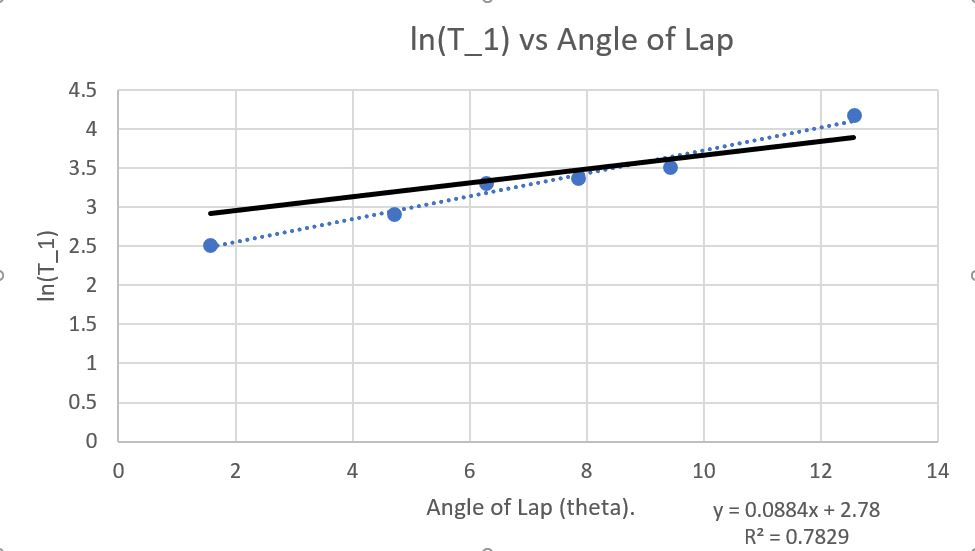
\includegraphics[width=1\textwidth]{chapters/lab2/graph1}
\caption{Equilibrium values of $\ln(T_1)$ vs $\theta$.}
\label{fig:mesh2}
\end{figure}
Drawing the line of best fit from the y-intercept then the equation of the line in terms of $\theta$ and $\ln(T_1)$ is given by:
\begin{equation}
\ln(T_1) = 0.0884\theta + 2.78 
\end{equation}

Therefore, the coefficient of friction $\mu$ is approximately 0.0884.



\subsection*{3.2 Analysis of V-Belft Friction Experiment.}
\addcontentsline{toc}{section}{3.2 Analysis of V-Belt Friction Experiment.}
In this section of experiment, vee-belt is used and in order to determine the coefficient of friction $\mu$, we start varying the tension on the slack side $T_2$ and then find the corresponding tension on the tight side $T_1$ until the belt starts to slip while maintaining a constant angle of lap $\theta$ to be $40\degree$ and $\alpha$ of $38\degree$. The results of the experiments are shown on the table below.
\begin{table}[H]
\begin{center}
\begin{tabular}{c|c|c|}
\cline{2-3}
 & $M_2$ (kg)                                             & $M_1$(kg)   \\ \cline{2-3} 
 & 0.65$\pm$0.1                                            & 1.62$\pm$0.1 \\ \cline{2-3} 
 & \begin{tabular}[c]{@{}c@{}}1.16\\ ±0.1\end{tabular} & 2.25±0.1 \\ \cline{2-3} 
 & 1.66$\pm$0.1                                            & 3.05$\pm$0.1 \\ \cline{2-3} 
 & 2.16$\pm$0.1                                            & 4.05$\pm$0.1 \\ \cline{2-3} 
 & 2.66$\pm$0.1                                            & 5.17$\pm$0.1 \\ \cline{2-3} 
 & 3.17$\pm$0.1                                                & 6.42$\pm$0.1 \\ \cline{2-3} 
\end{tabular}
\caption{Vee belt friction experiment results.}
\label{tab: 9}
\end{center}
\end{table}

Multiplying the mass by the acceleration due to gravity and applying the same uncertainty equation as experiment above, then the tension for both the slack side and the tight side are given on the table below:
\begin{table}[H]
\begin{center}
\begin{tabular}{c|c|c|}
\cline{2-3}
 & $T_2$ (N)                                             & $T_1$(N)   \\ \cline{2-3} 
 & 6.37$\pm$0.98                                            & 15.9$\pm$0.98 \\ \cline{2-3} 
 & \begin{tabular}[c]{@{}c@{}}11.36$\pm$0.99\end{tabular} & 22.04$\pm$0.98 \\ \cline{2-3} 
 & 16.26$\pm$0.98                                            & 29.87$\pm$0.98 \\ \cline{2-3} 
 & 21.16$\pm$0.98                                            & 39.67$\pm$0.98 \\ \cline{2-3} 
 & 26.05$\pm$0.98                                            & 50.63$\pm$0.98 \\ \cline{2-3} 
 & 31.05$\pm$0.98                                                & 62.88$\pm$0.98\\ \cline{2-3} 
\end{tabular}
\caption{Tension of the vee belt.}
\label{tab: 10}
\end{center}
\end{table}

The graph of $T_2$ versus $T_1$ is shown below:
\begin{figure}[H]
\centering
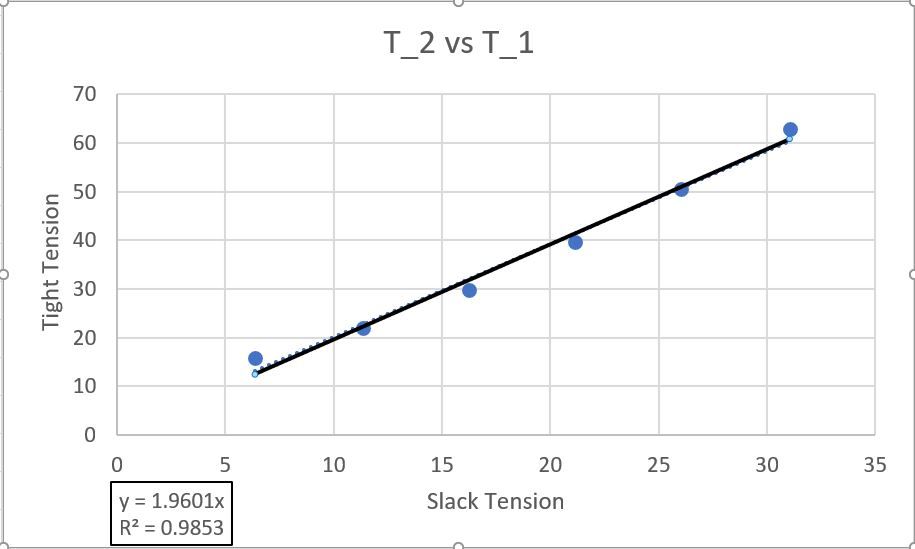
\includegraphics[width=1\textwidth]{chapters/lab2/m2}
\caption{$T_2$ versus $T_1$ graph.}
\label{fig:mesh3}
\end{figure}

The line of best fit of above graph has a gradient of 1.9601. To deduce $\mu$, we must calculate $\mu '$ first. Rearranging equation 6 to find $\mu '$, then $\mu'$ is given by:
\begin{align}
\mu ' &= \frac{1}{\theta}\ln\left(\frac{\delta T_1}{\delta T_2}\right) \notag
\end{align}
Where $\frac{\delta T_1}{\delta T_2}$ is equal to the gradient of the line of best fit above. Substituting all the required value into above equation, then $\mu '$ value to three significant figures calculated to be:
\begin{align}
\mu ' &= \frac{180}{40\pi}\ln\left(1.9601\right) \notag \\
\qquad &= 7.57\times10^{-1} \notag
\end{align}

Substituting the value of $\mu '$ and $\alpha$ into equation 7, then the $\mu$ to three significant is given by:
\begin{align}
\mu &= \mu ' * \cos(0.5\alpha) \notag \\
\qquad &= 0.757* \cos(0.5*\frac{38\pi}{180}) \notag \\
\qquad &=  0.716 \notag
\end{align}
\subsection*{3.3 Discussion.}
\addcontentsline{toc}{section}{3.3 Discussion.}
The graph on the figure 6 has a $R^2$ value of $0.7829$ which mean $70\%$ of the experimental data fits the linear regression line. On the other hand, the graph on figure 7 has a $R^2$ value of approximately $0.99$ which mean $99\%$ of the experimental data for vee belt resembles the linear regression line from origin. The source of error for this experiment comes from systematic errors that happen during experiment such as the weight balance is not "zero" properly, the angle of lap is not exactly what it meant to be. Moreover, random errors also happen during the experiment and it is something that we cannot control. These errors such as the humidity of the room might coat the surface of the drum with small amount of water therefore causing the coefficient of friction of the drum's surface to either decrease or increase. \\

The experimental results above show limiting slip conditions for each belt types (coil and vee-belt) that were used in the experiment. The limiting slip condition values showed the maximum power that can be transmitted into the belt without slipping. The theoretical relationship can be proven by substituing the value of $T_2$, $\mu$, and $\theta$ into the equation $T_1 = e^{\theta \mu}T_2$ for coil belt and substituting the value of  $T_2$, $\mu$, $\theta$ and $\alpha$ into  $T_1 = e^{\theta \mu '}T_2$ and $\mu = \mu ' \csc\left(\frac{\alpha}{2}\right)$.

\section*{4.0 Epicyclic Gear.}
\addcontentsline{toc}{chapter}{4.0 Epicyclic Gear.}
The objectives of this experiment are to familiarise ourself with epicyclic gearing system and experimentally analytically determine the velocity ratios of epicyclic gear system by making the carrier arm, annulus gear, and sun gear fixed one at a time. The apparatus for this experiment consists of four gears as seen on the image below and individual shafts are able to be locked independently in order for us to carry the experiment. \\
\begin{figure}[H]
\centering
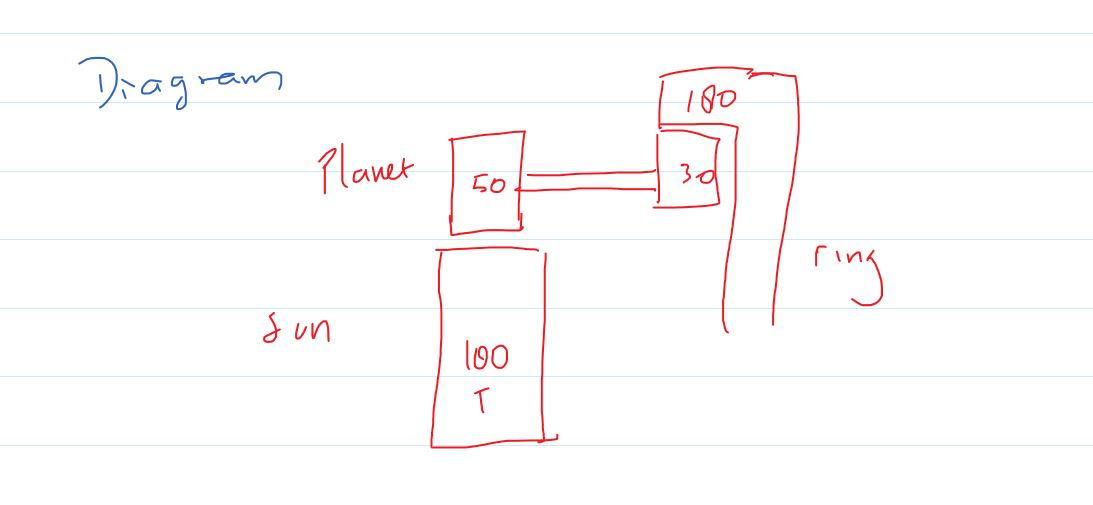
\includegraphics[width=1\textwidth]{chapters/lab3/geardrawing}
\caption{Epicyclic gear drawing.}
\label{fig:mesh1}
\end{figure}
This experiment is divided into three parts with the first part is to determine the speed ratio between the input shaft (sun gear) and the output shaft (annulus gear). The second part also to determine the velocity ratio between input and output shafts (sun and the carrier arm) with the annulus or ring gear is fixed. The last part is to determine the velocity ratio between the carrier arm (input) and the annulus gear or the ring gear (output). However, in this part, the sun gear is fixed. \\

In this experiment the constants are the number of teeth and it is shown below:
\begin{itemize}
\item $T_{sun}$ = 100 Teeth.
\item $T_{planet_1}$ = 50 Teeth.
\item $T_{planet_2}$ = 30 Teeth.
\item $T_{ring}$ = 180 Teeth.
\end{itemize}
Where $T_{planet_1}$ is the planet gear that is meshing to the sun gear and $T_{planet_2}$ is the planet gear that is meshing with the ring gear.
\subsection*{4.1 Speed Ratio Analysis for Fixed Carrier Arm.}
\addcontentsline{toc}{section}{4.1 Speed Ratio Analysis for Fixed Carrier Arm.}
For this part, if we were to rotate the sun gear one full rotation clockwise, then the planet gear that mesh with the sun gear, $planet_1$ will rotate twice in the opposite direction (anti-clockwise). The planet gear that meshes with the annulus or ring gear $Planet_2$ will cause the ring gear to rotate only $\frac{1}{3}$ and its motion is on the opposite direction to the planet gear (clockwise direction).\\

Therefore, the velocity ratio between the input gear and the sun gear is given by:
\begin{align}
\frac{Input Gear}{Output Gear} &= \frac{1}{\frac{1}{3}} \notag \\
\qquad &= \frac{3}{1} \notag
\end{align}
Therefore, the input and the output gear has a ratio of $3:1$ or $1:\frac{1}{3}$.
\subsection*{4.2 Speed Ratio Analysis for Fixed Annulus Gear.}
\addcontentsline{toc}{section}{4.2 Speed Ratio Analysis for Fixed Annulus Gear.}
\begin{table}[H]
\begin{tabular}{|c|c|c|c|c|}
\hline
Components                         & Planets & Carrier Arm & Sun Gear & Ring Gear \\ \hline
\begin{tabular}[c]{@{}c@{}}Lock all components \\ and rotate +1.\end{tabular} & $+$1      & $+$1          & $+$1       & $+$1        \\ \hline
\begin{tabular}[c]{@{}c@{}}Lock the arm and \\ rotate the ring gear -1 \\ to give the fixed ring gear.\end{tabular} & $\frac{-180}{30}$ & 0 & $\left(\frac{-180}{30}\right)\left(\frac{-50}{100}\right)$ & $-$1 \\ \hline
Sum up the total motion.           & $-$5      & $+$1          & $+$4       & 0         \\ \hline
\end{tabular}
\caption{Tabular method for fixed ring gear.}
\label{tab:12}
\end{table}

Concluding from the table above ratio between the input shaft (sun) and the output shaft (carrier arm) is given by:
\begin{align}
\frac{input}{output} &= \frac{4}{1} \notag
\end{align}
\subsection*{4.3 Speed Ratio Analysis for Fixed Sun Gear.}
\addcontentsline{toc}{section}{4.3 Speed Ratio Analysis for Fixed Sun Gear.}
\begin{table}[H]
\begin{tabular}{|c|c|c|c|c|}
\hline
Components                         & Planets & Carrier Arm & Sun Gear & Ring Gear \\ \hline
\begin{tabular}[c]{@{}c@{}}Lock all component \\ together and rotate +1.\end{tabular}  & $+$1      & $+$1          & $+$1       & $+$1        \\ \hline
\begin{tabular}[c]{@{}c@{}}Lock the arm and \\ rotate the sun gear -1 \\ to give the fixed sun gear.\end{tabular} & $-1\frac{-100}{50}$ & 0 & $-1$ &$\left(\frac{100}{50}\right)\left(\frac{30}{180}\right)$ \\ \hline
Sum up the total motion.           & $-$3      &  0          & $+$1       & $\frac{4}{3}$         \\ \hline
\end{tabular}
\caption{Tabular method for fixed sun gear.}
\label{tab:13}
\end{table}

Concluding from the table above ratio between the input shaft (carrier arm) and the output shaft (annulus gear) is given by:
\begin{align}
\frac{input}{output} &= \frac{1}{\frac{4}{3}} \notag \\
\qquad &= \frac{3}{4} \notag
\end{align}
\section*{5.0 Conclusion}
\addcontentsline{toc}{chapter}{5.0 Conclusion.}
The goal of the experiments is to analyse for each experiment the experimental results gathered using theoretical knowledge gained from the lecture slides as well as formulae or equations that were included in the laboratory script. The methods used for the first experiment were the compound pendulum method and the trifilar suspension method. The method use for the second
experiment was to add mass to the slack side of the belt and then add small amount of mass to the tight side of the belt until the belt starts to slip. Lastly, the method used for the third experiment was the tabular method to determine the speed ratio between the input and the output.\\

The moment of inertia of the object from the first experiment comes out to be 0.035 $kg.m^2$ with uncertainty of approximately 2$\%$ using the trifilar method and 0.033 $kg.m^2$ with uncertainty of approximately $9\%$ using the compound pendulum method. For the second experiment, the coefficient of friction $\mu$ comes out to be 0.884 for the coil belt and 0.716 for the vee-belt configuration. Lastly, the speed ratio when the carrier arm is fixed is 3 to 1, 4 to 1 when the annulus or ring gear is fixed and 3 to 4 when the sun gear is fixed.\\

The first experiment is considered to be successful because the uncertainty calculated is less than $10\%$. In addition to that, the second experiment is also considered to be successful because based on the $R^2$ value, the experimental data represent $99\%$ and above $70\%$ of the linear regression line. 
\pagebreak
\section*{6.0 References.}
\addcontentsline{toc}{chapter}{6.0 References.}
\begin{enumerate}
\item Hinrichsen, Peter. 2015. "Analysis of Bi and Trifilar Oscillations.".\url{https://www.researchgate.net/publication/277404917_Analysis_of_Bi_and_Trifilar_Oscillations}.
\item Hinrichsen, Peter. 2016. "Trifilar Suspension Centering Correction." \url{https://www.researchgate.net/publication/303614060_Trifilar_Suspension_Centering_Correction}.
\item Du Bois, Jonathan $\&$ Lieven, Naj $\&$ Adhikari, Sondipon. 2009. "Error Analysis in Trifilar Inertia Measurements. Experimental Mechanics". \url{https://www.researchgate.net/publication/226018805_Error_Analysis_in_Trifilar_Inertia_Measurements}.
\item ckit. n.d. "Belt Tension Theory: Factors". Accessed May 29,2020. \url{https://www.ckit.co.za/secure/conveyor/troughed/belt_tension/belt_tension_factors.htm}.
\item Howard, Ian. 2020. Moment of inertia experiemental results. Dataset. Curtin University. \\ \url{https://lms.curtin.edu.au/bbcswebdav/pid-7423774-dt-content-rid-43761563_1/xid-43761563_1}
\item Howard, Ian. 2020. Belt Friction experiemental results. Dataset. Curtin University. \\ \url{https://lms.curtin.edu.au/bbcswebdav/pid-7423772-dt-content-rid-43761564_1/xid-43761564_1}
\item Howard, Ian. 2020. "Epicyclic Gear Lab Demonstration Video". Video. Curtin University Machine Dynamics BlackBoard.
\item Howard, Ian. 2020. "MassMomentOfInertia Part A - CompoundPendulumExperiment". mp4 video. Curtin University Machine Dynamics BlackBoard.
\item Howard, Ian. 2020. "MassMomentOfInertia Part B - TriFilar Suspension". mp4 video. Curtin University Machine Dynamics BlackBoard.
\item Howard, Ian. 2020. "Experimental Error Analysis Video". Video. Curtin University Machine Dynamics BlackBoard.
\item Howard, Ian. 2020. "Belt Friction Demostration Laboratory Video". Video. Curtin University Machine Dynamics BlackBoard.
\end{enumerate}
\appendix
\section*{7.0 Appendices.}
\addcontentsline{toc}{chapter}{7.0 Appendices.}
\subsection*{7.1 Moment of Inertia Laboratory Script.}
\addcontentsline{toc}{section}{7.1 Moment of Inertia Laboratory Script.}
\begin{figure}[H]
  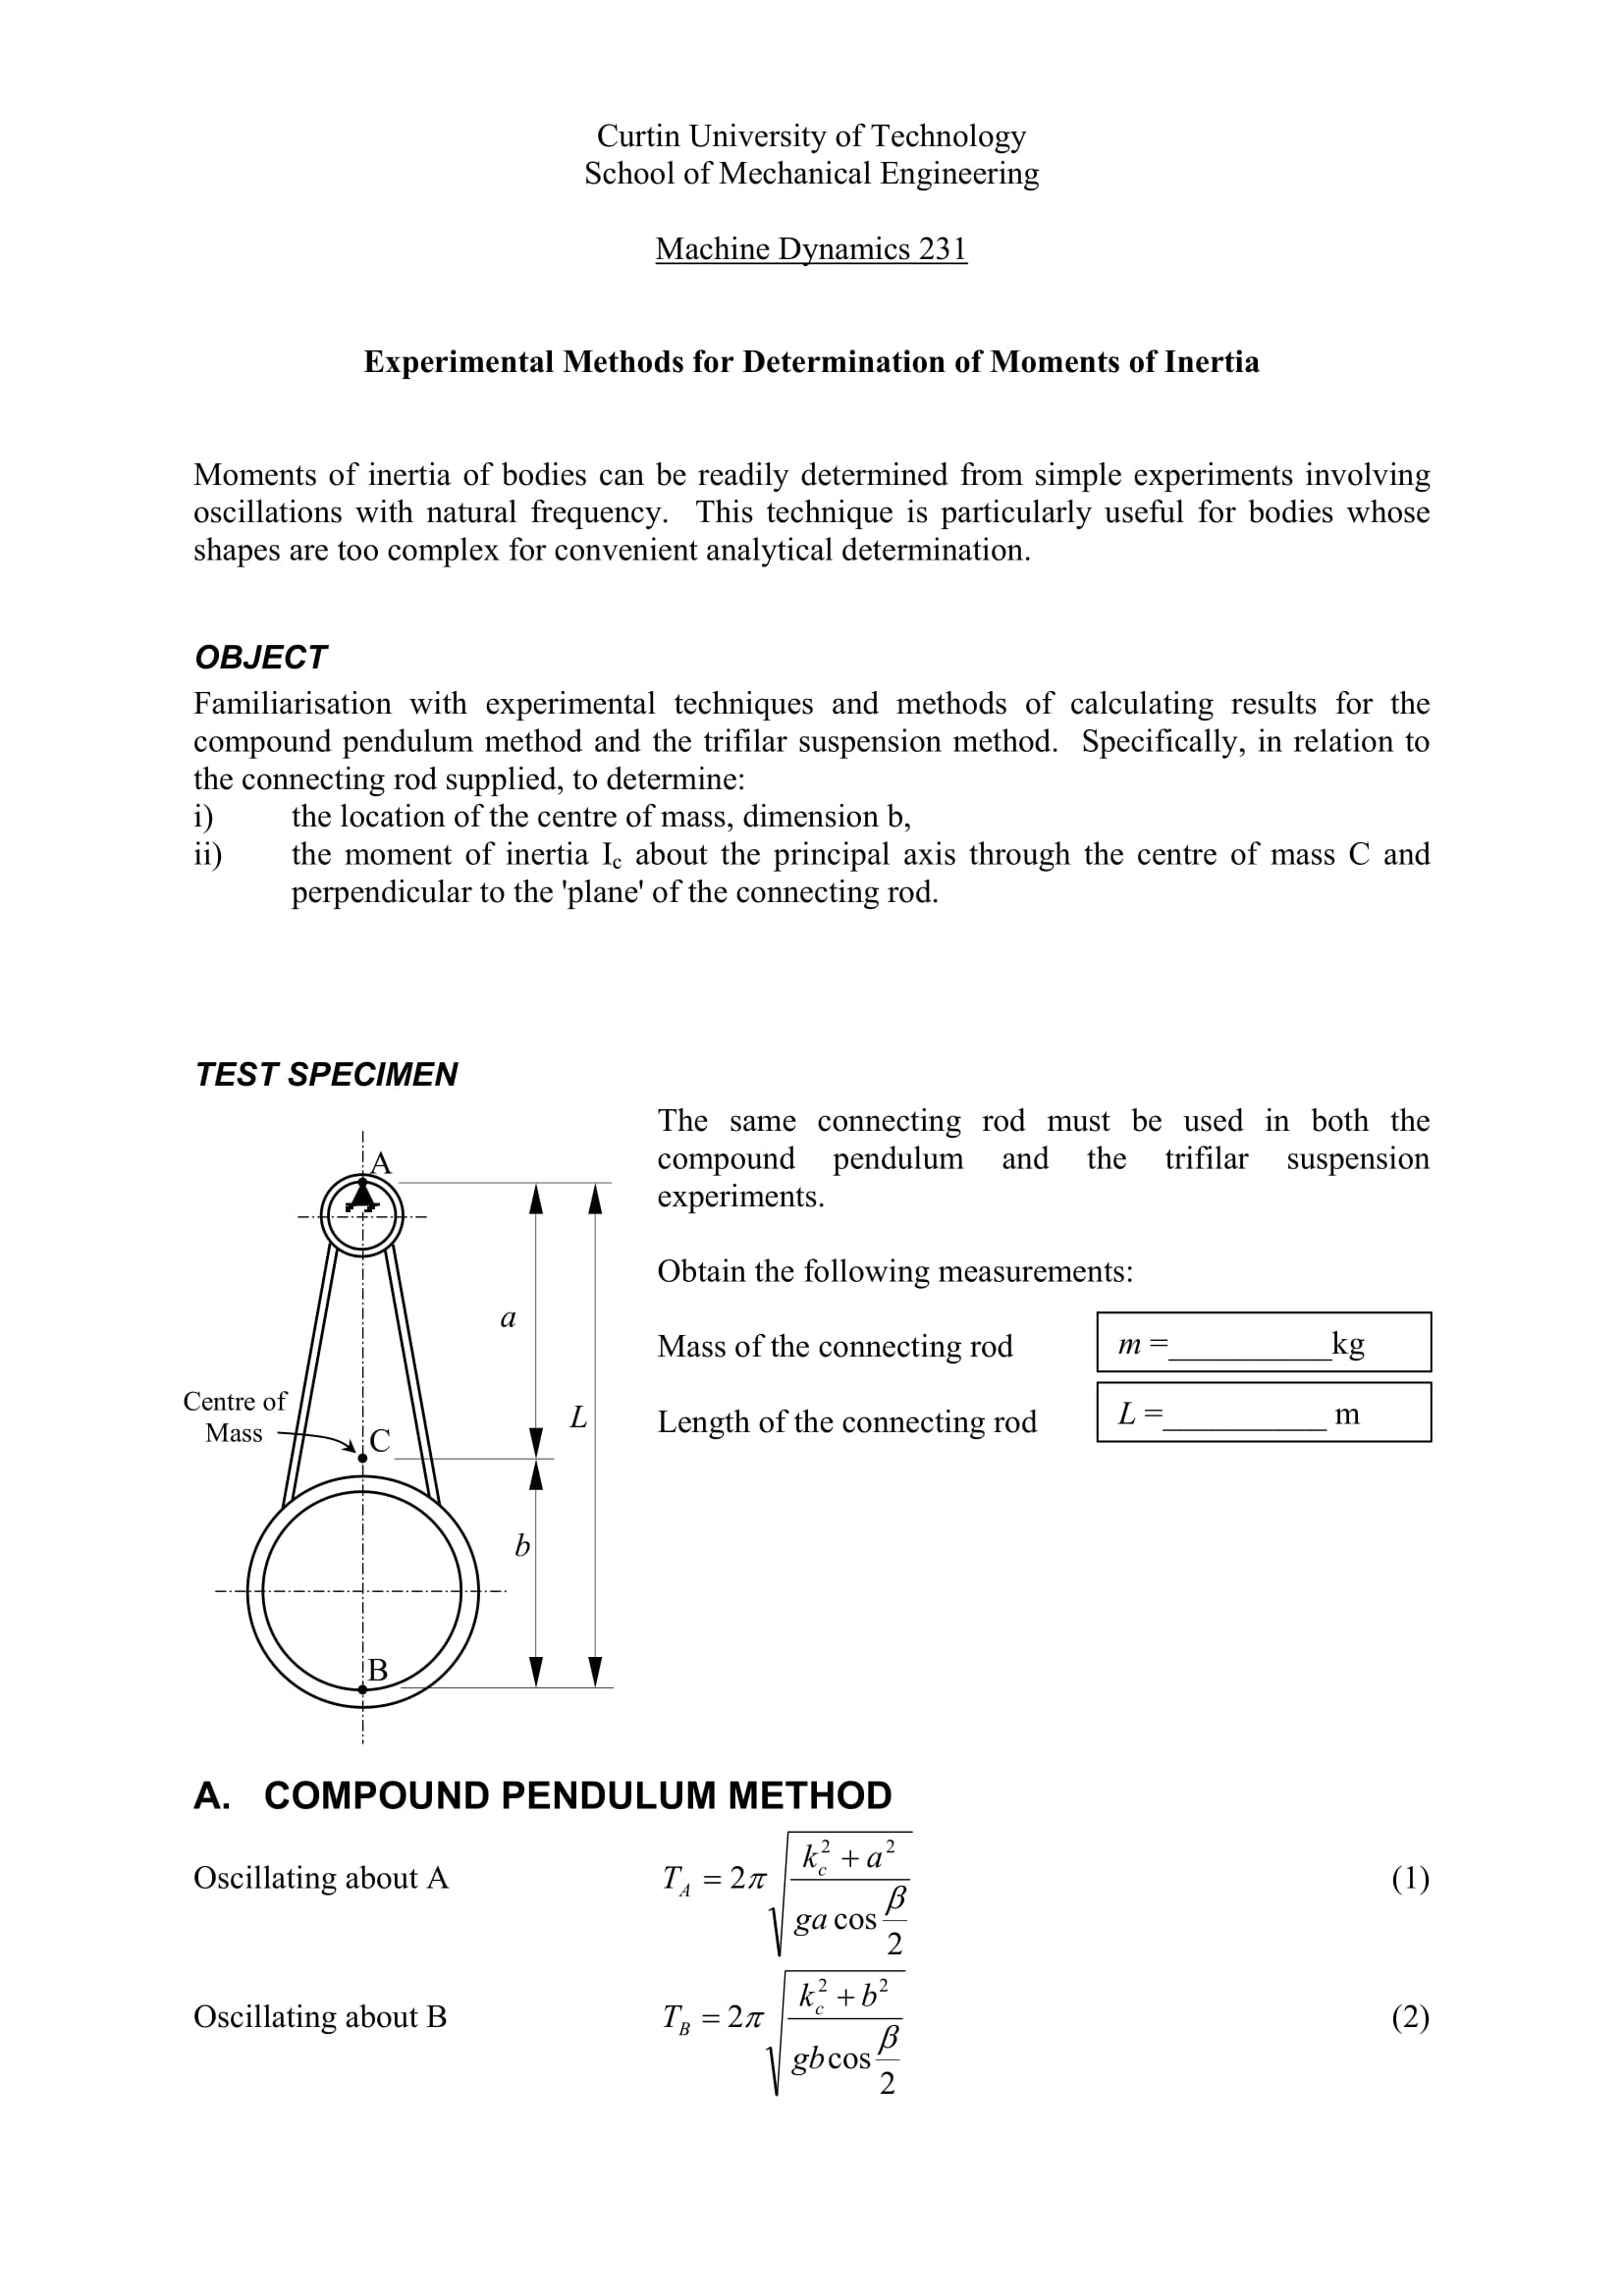
\includegraphics[width=\linewidth]{lab1/lab1-1}
  \caption*{}
\label{}
\end{figure}
\begin{figure}
 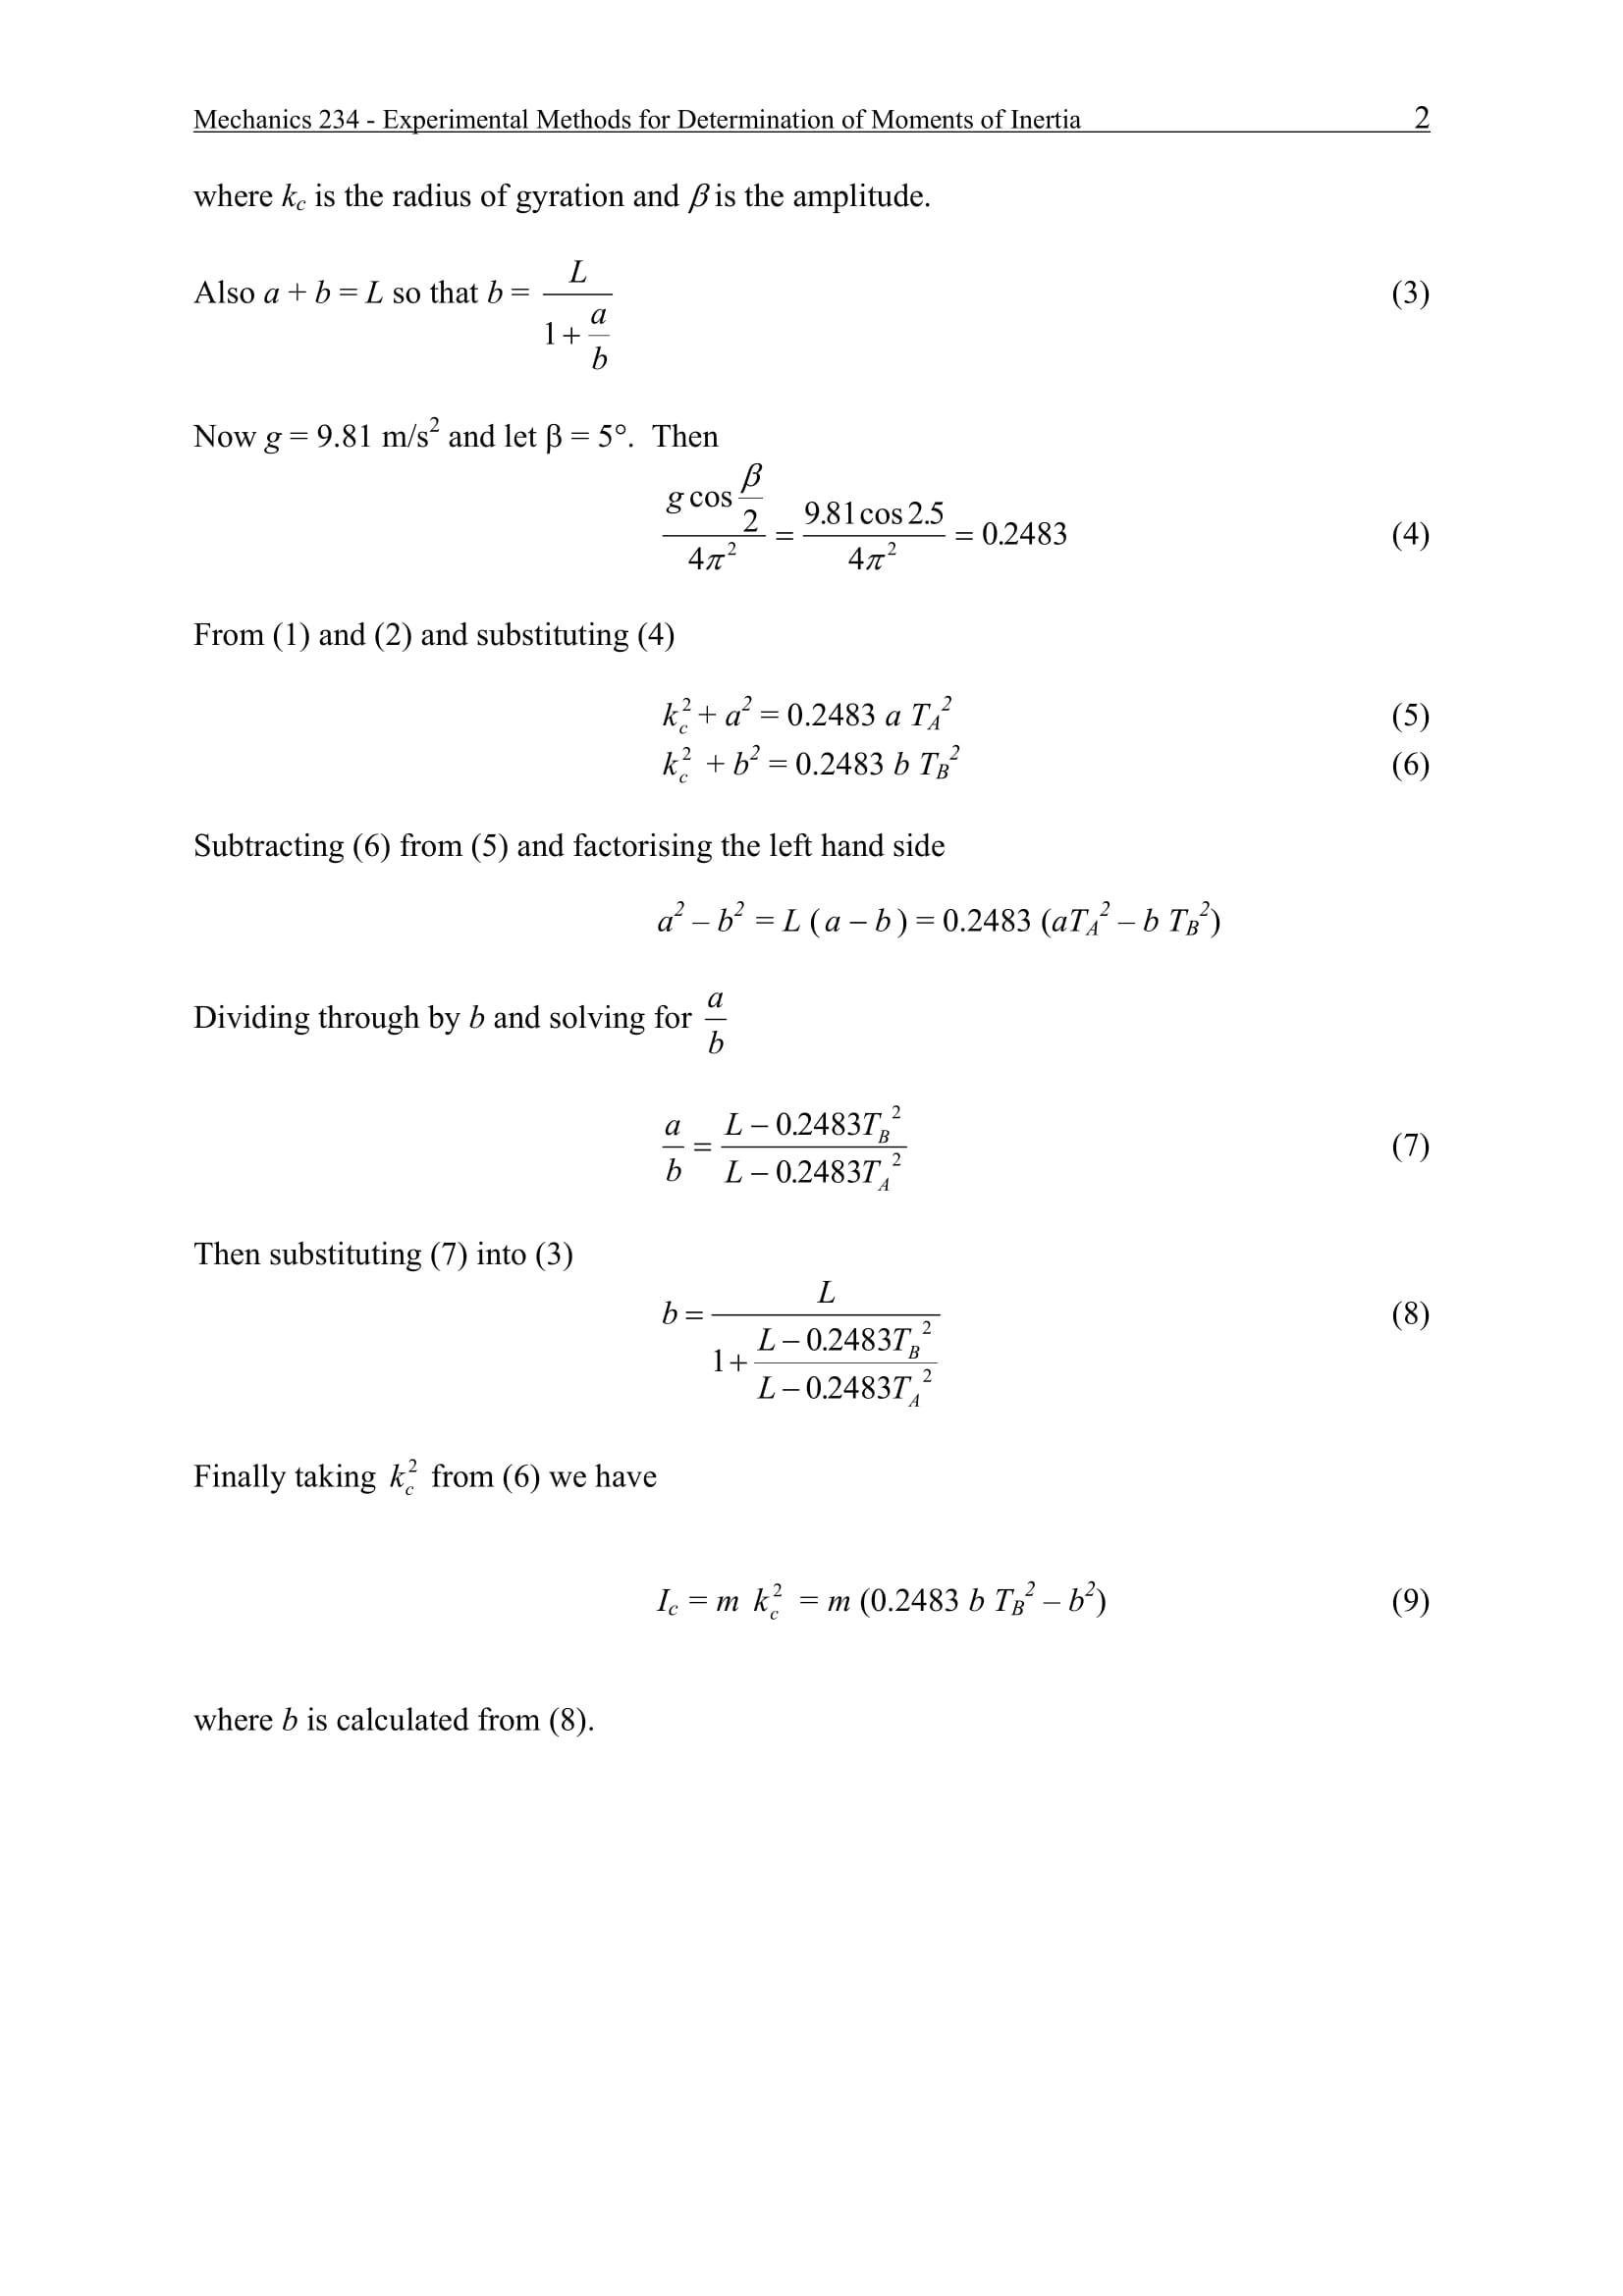
\includegraphics[width=\linewidth]{lab1/lab1-2}
  \caption*{}
\label{}
\end{figure}
\begin{figure}
 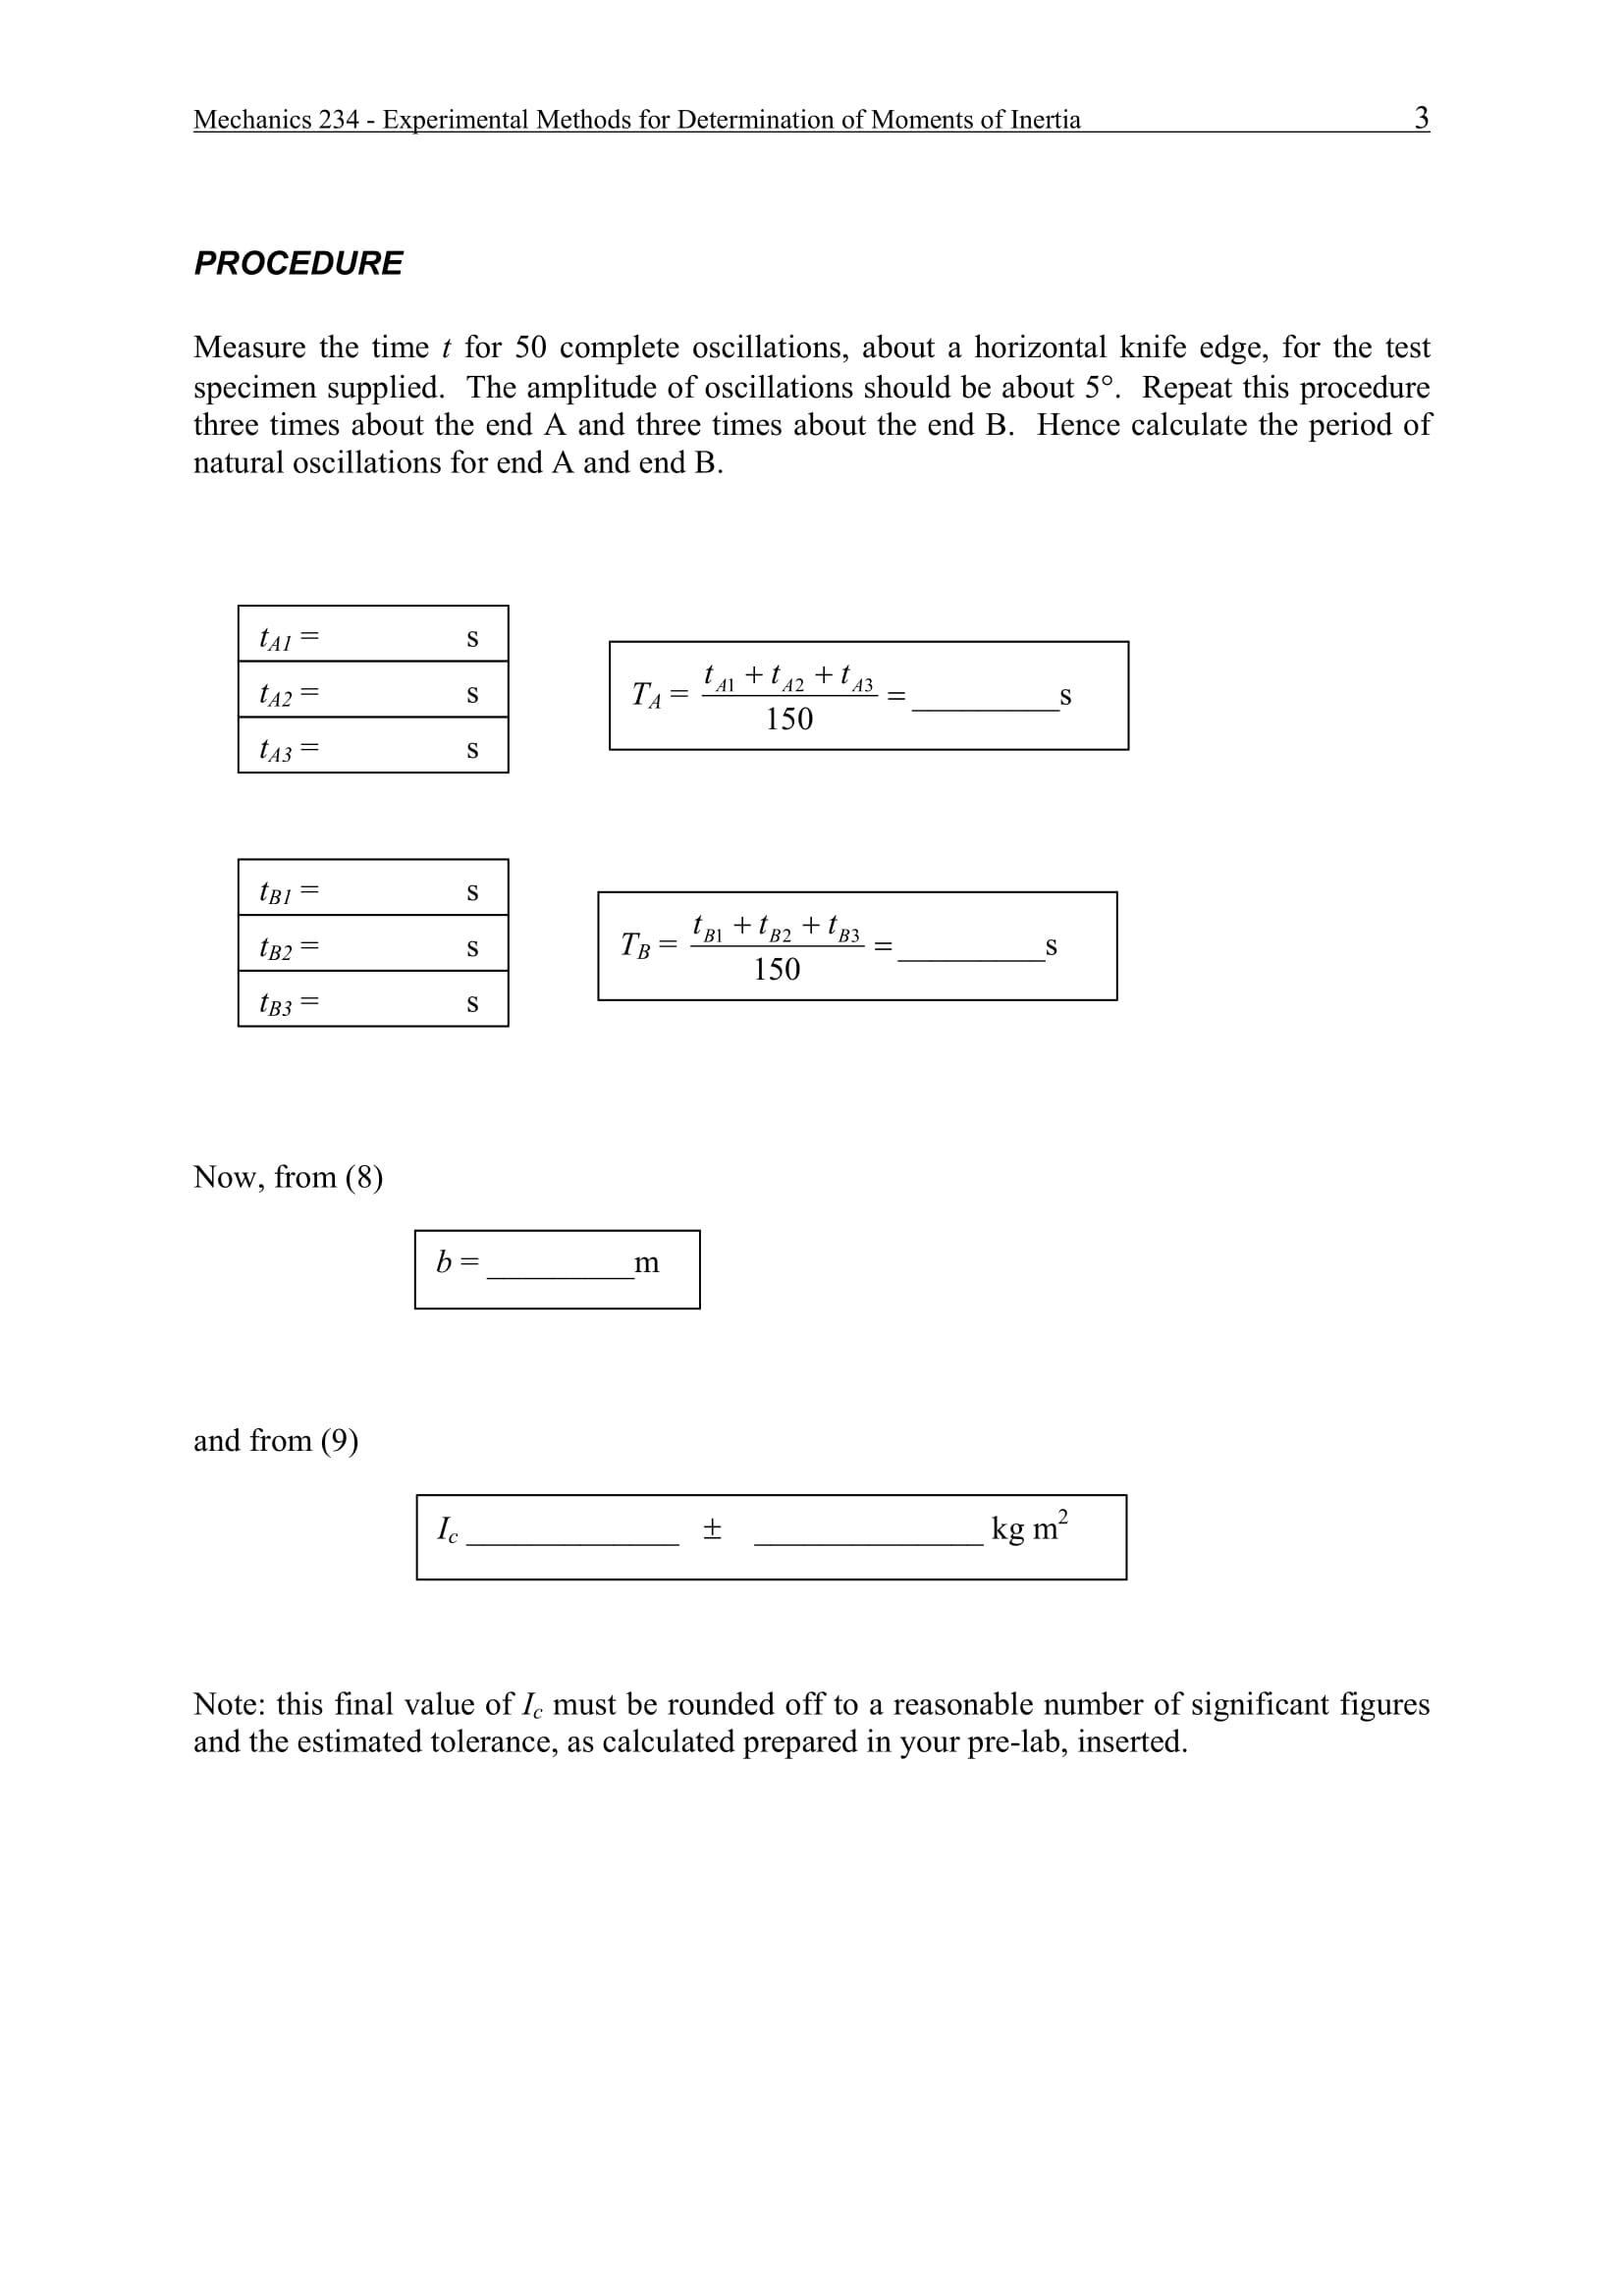
\includegraphics[width=\linewidth]{lab1/lab1-3}
  \caption*{}
\label{}
\end{figure}
\begin{figure}
 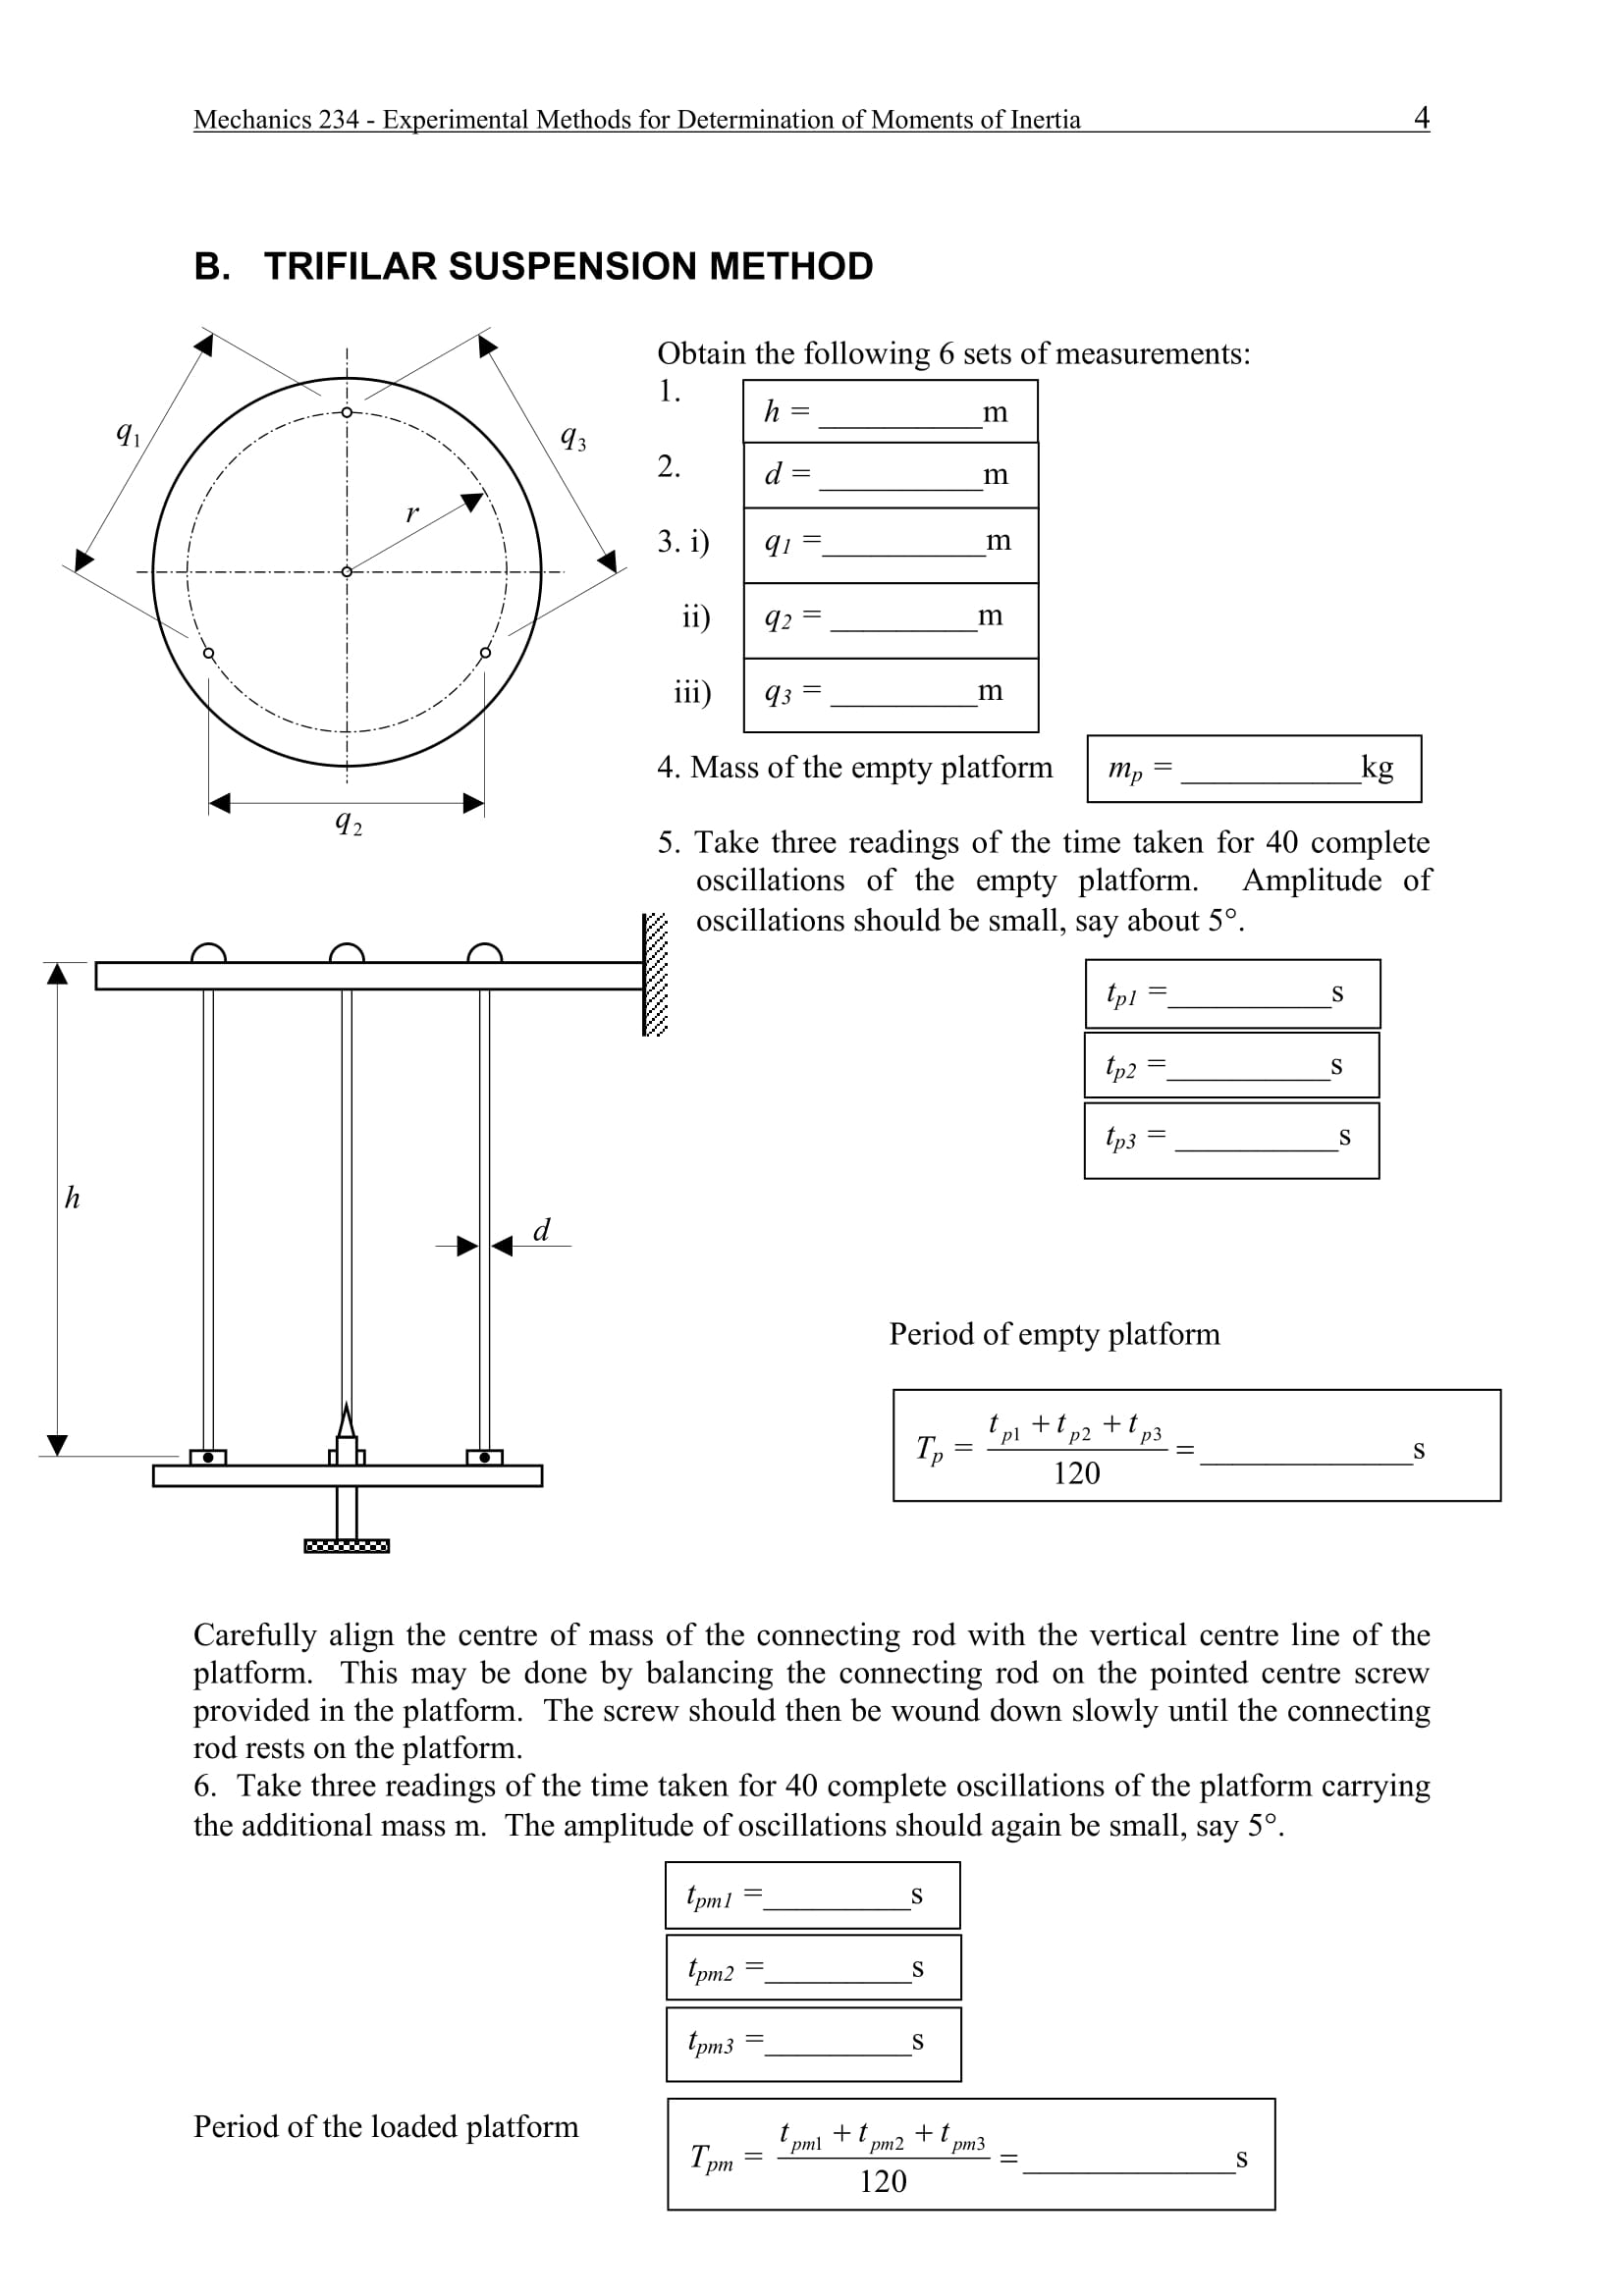
\includegraphics[width=\linewidth]{lab1/lab1-4}
  \caption*{}
\label{}
\end{figure}
\begin{figure}
 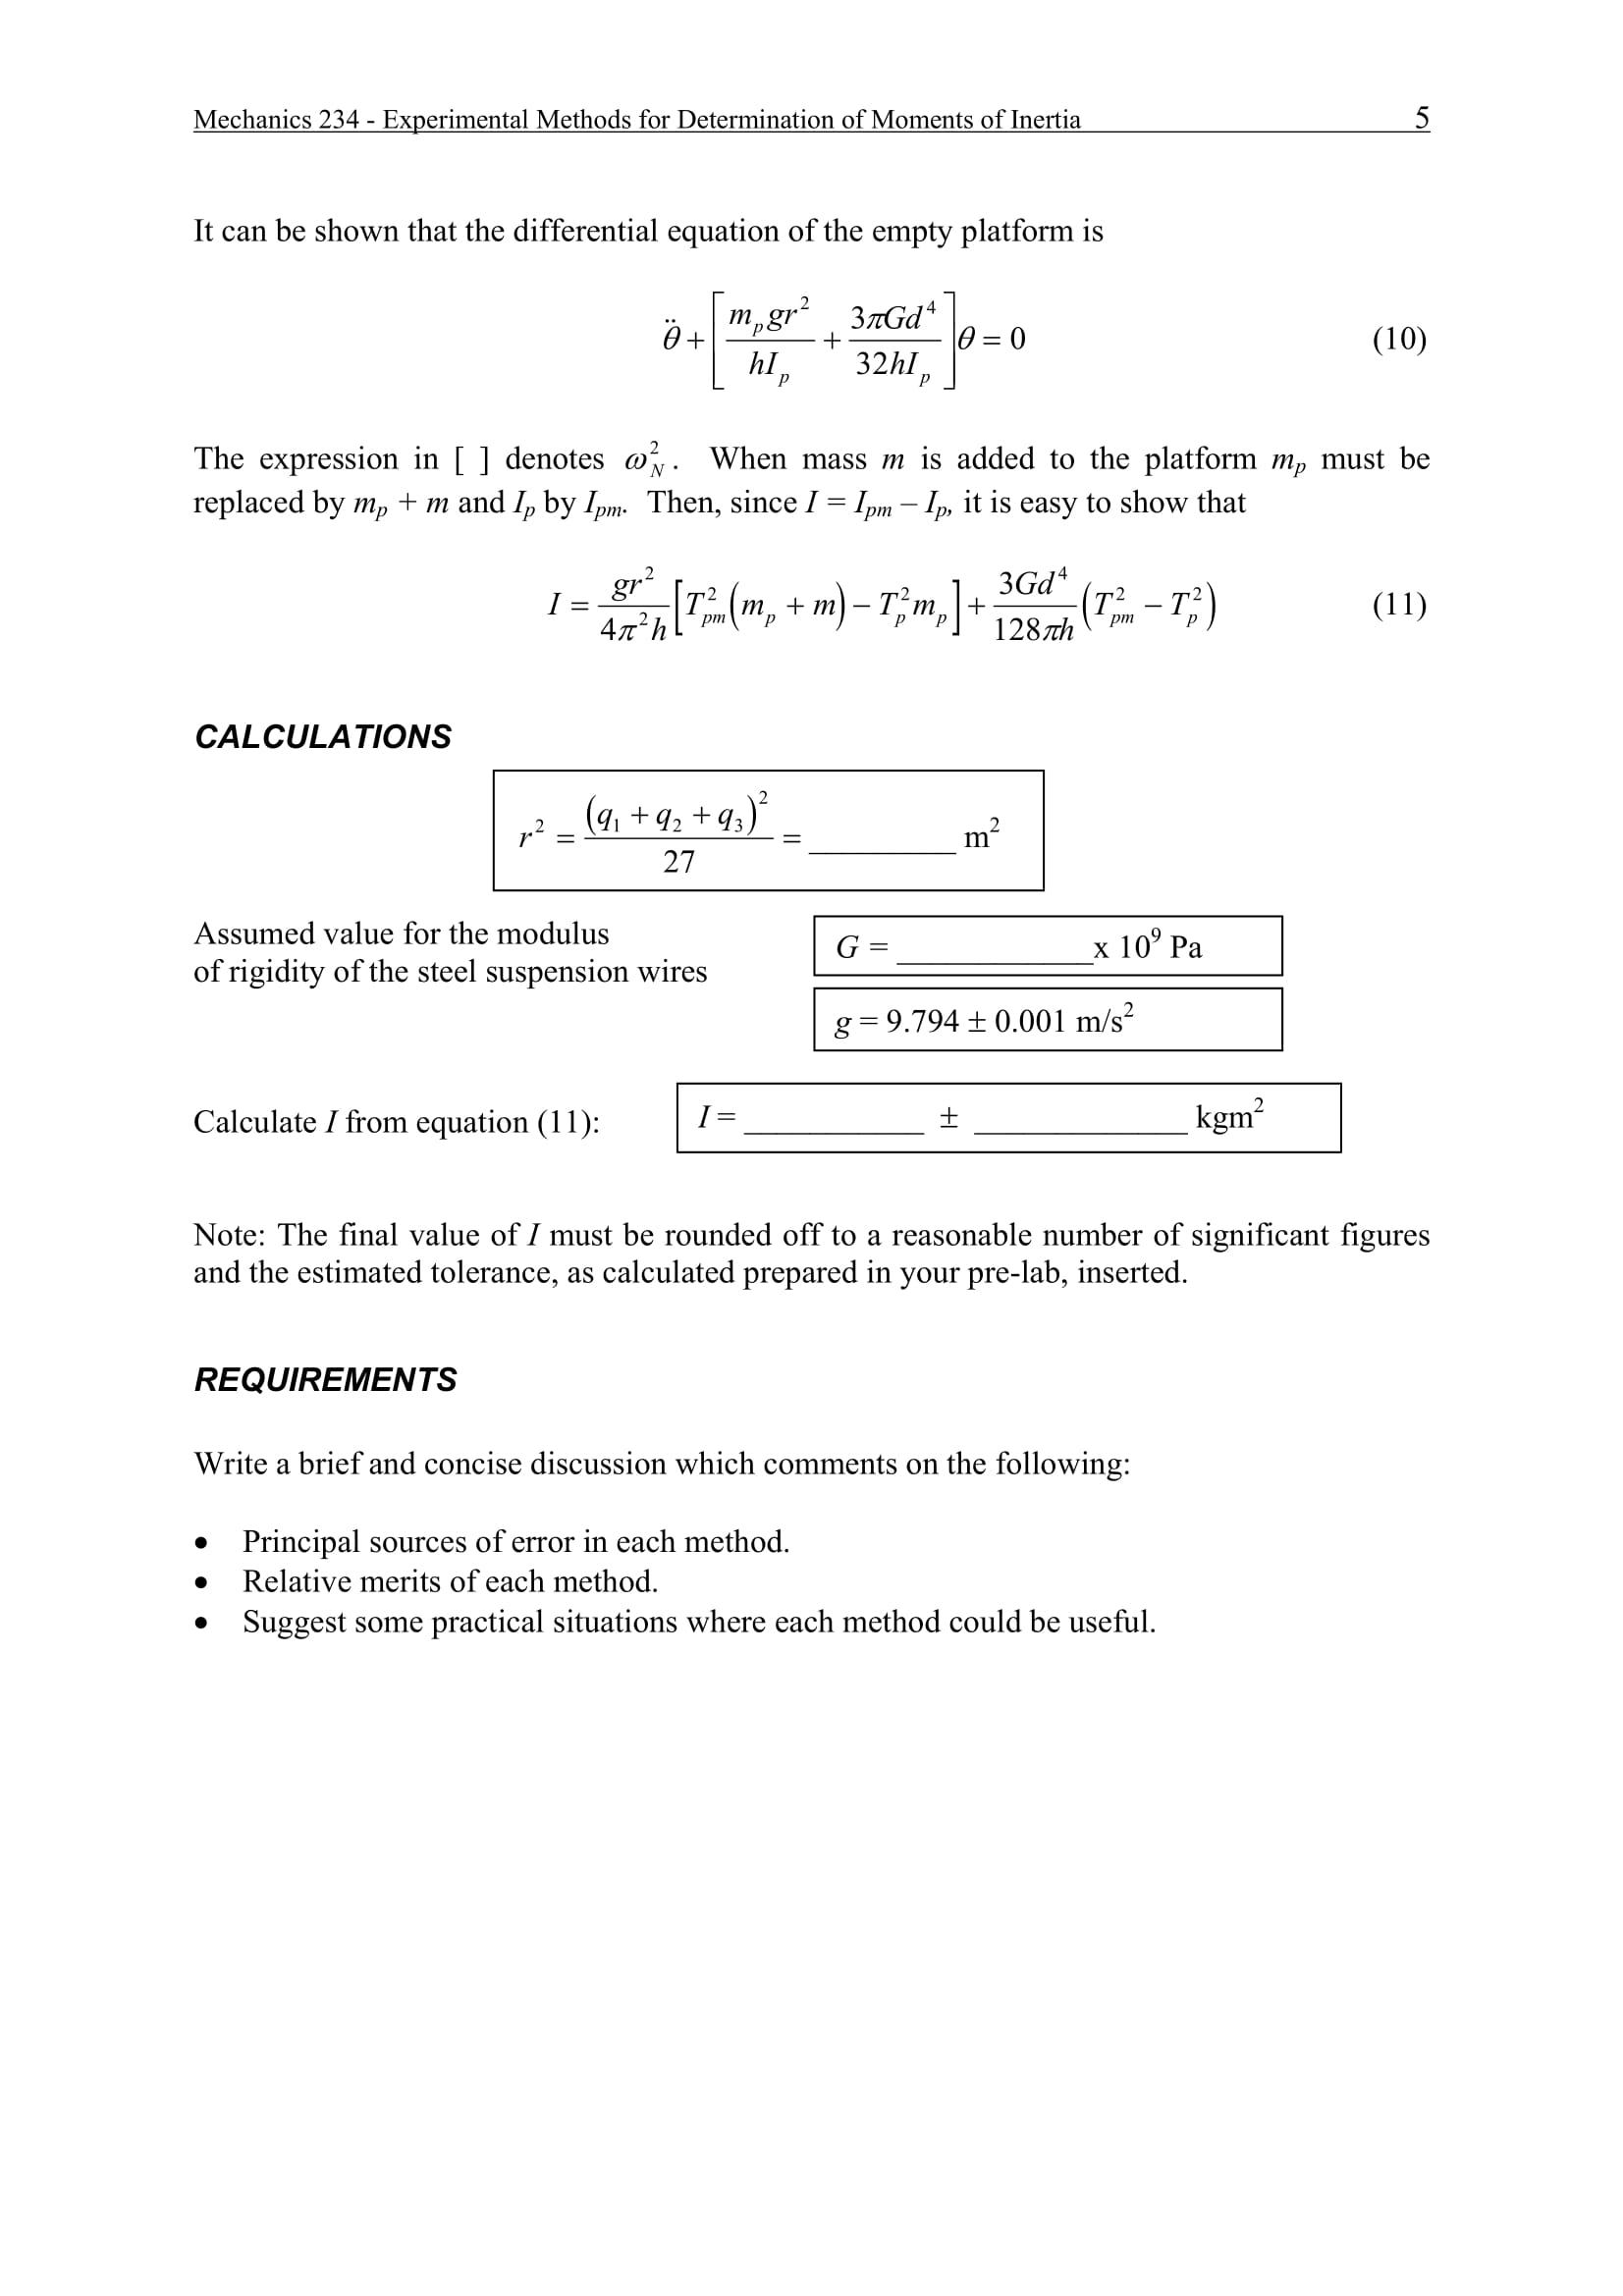
\includegraphics[width=\linewidth]{lab1/lab1-5}
  \caption*{}
\label{}
\end{figure}

\subsection*{7.2  Experimental Results for Moment of Inertia Experiment.}
\addcontentsline{toc}{section}{7.2  Experimental Results for Moment of Inertia Experiment.}
\begin{figure}[H]
  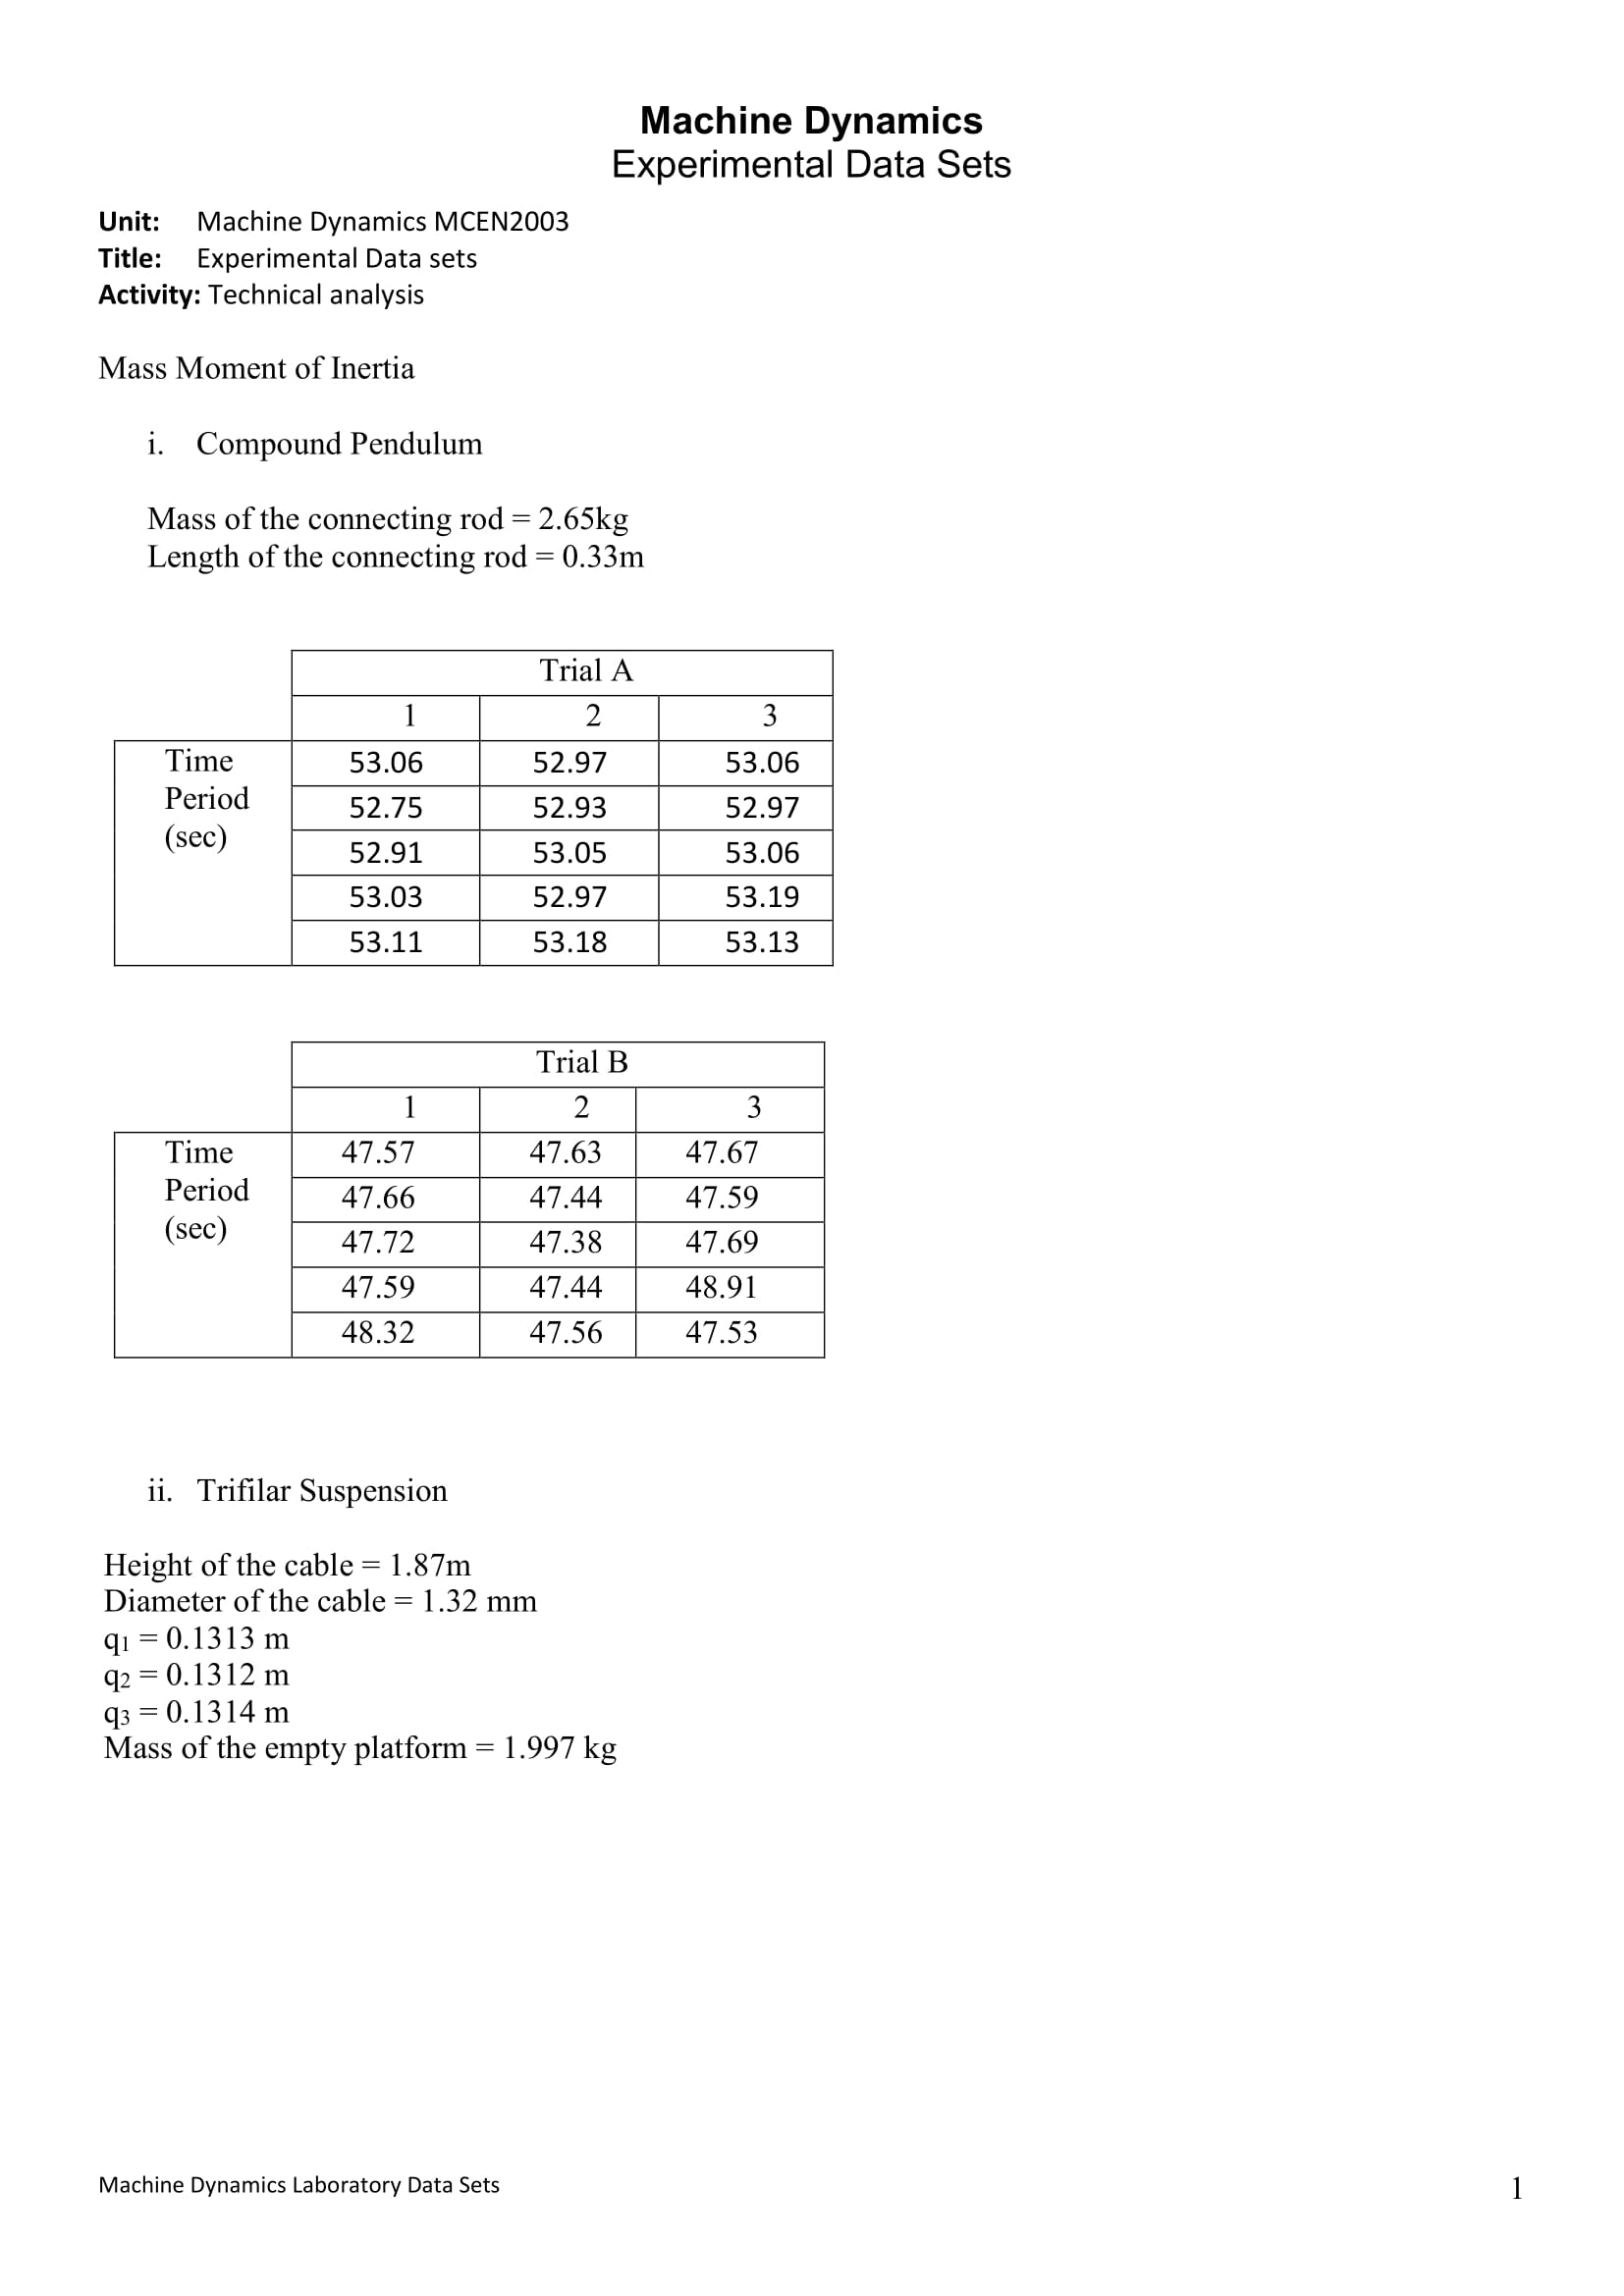
\includegraphics[width=\linewidth]{dataset/mass1}
  \caption*{}
\label{}
\end{figure}
\begin{figure}
  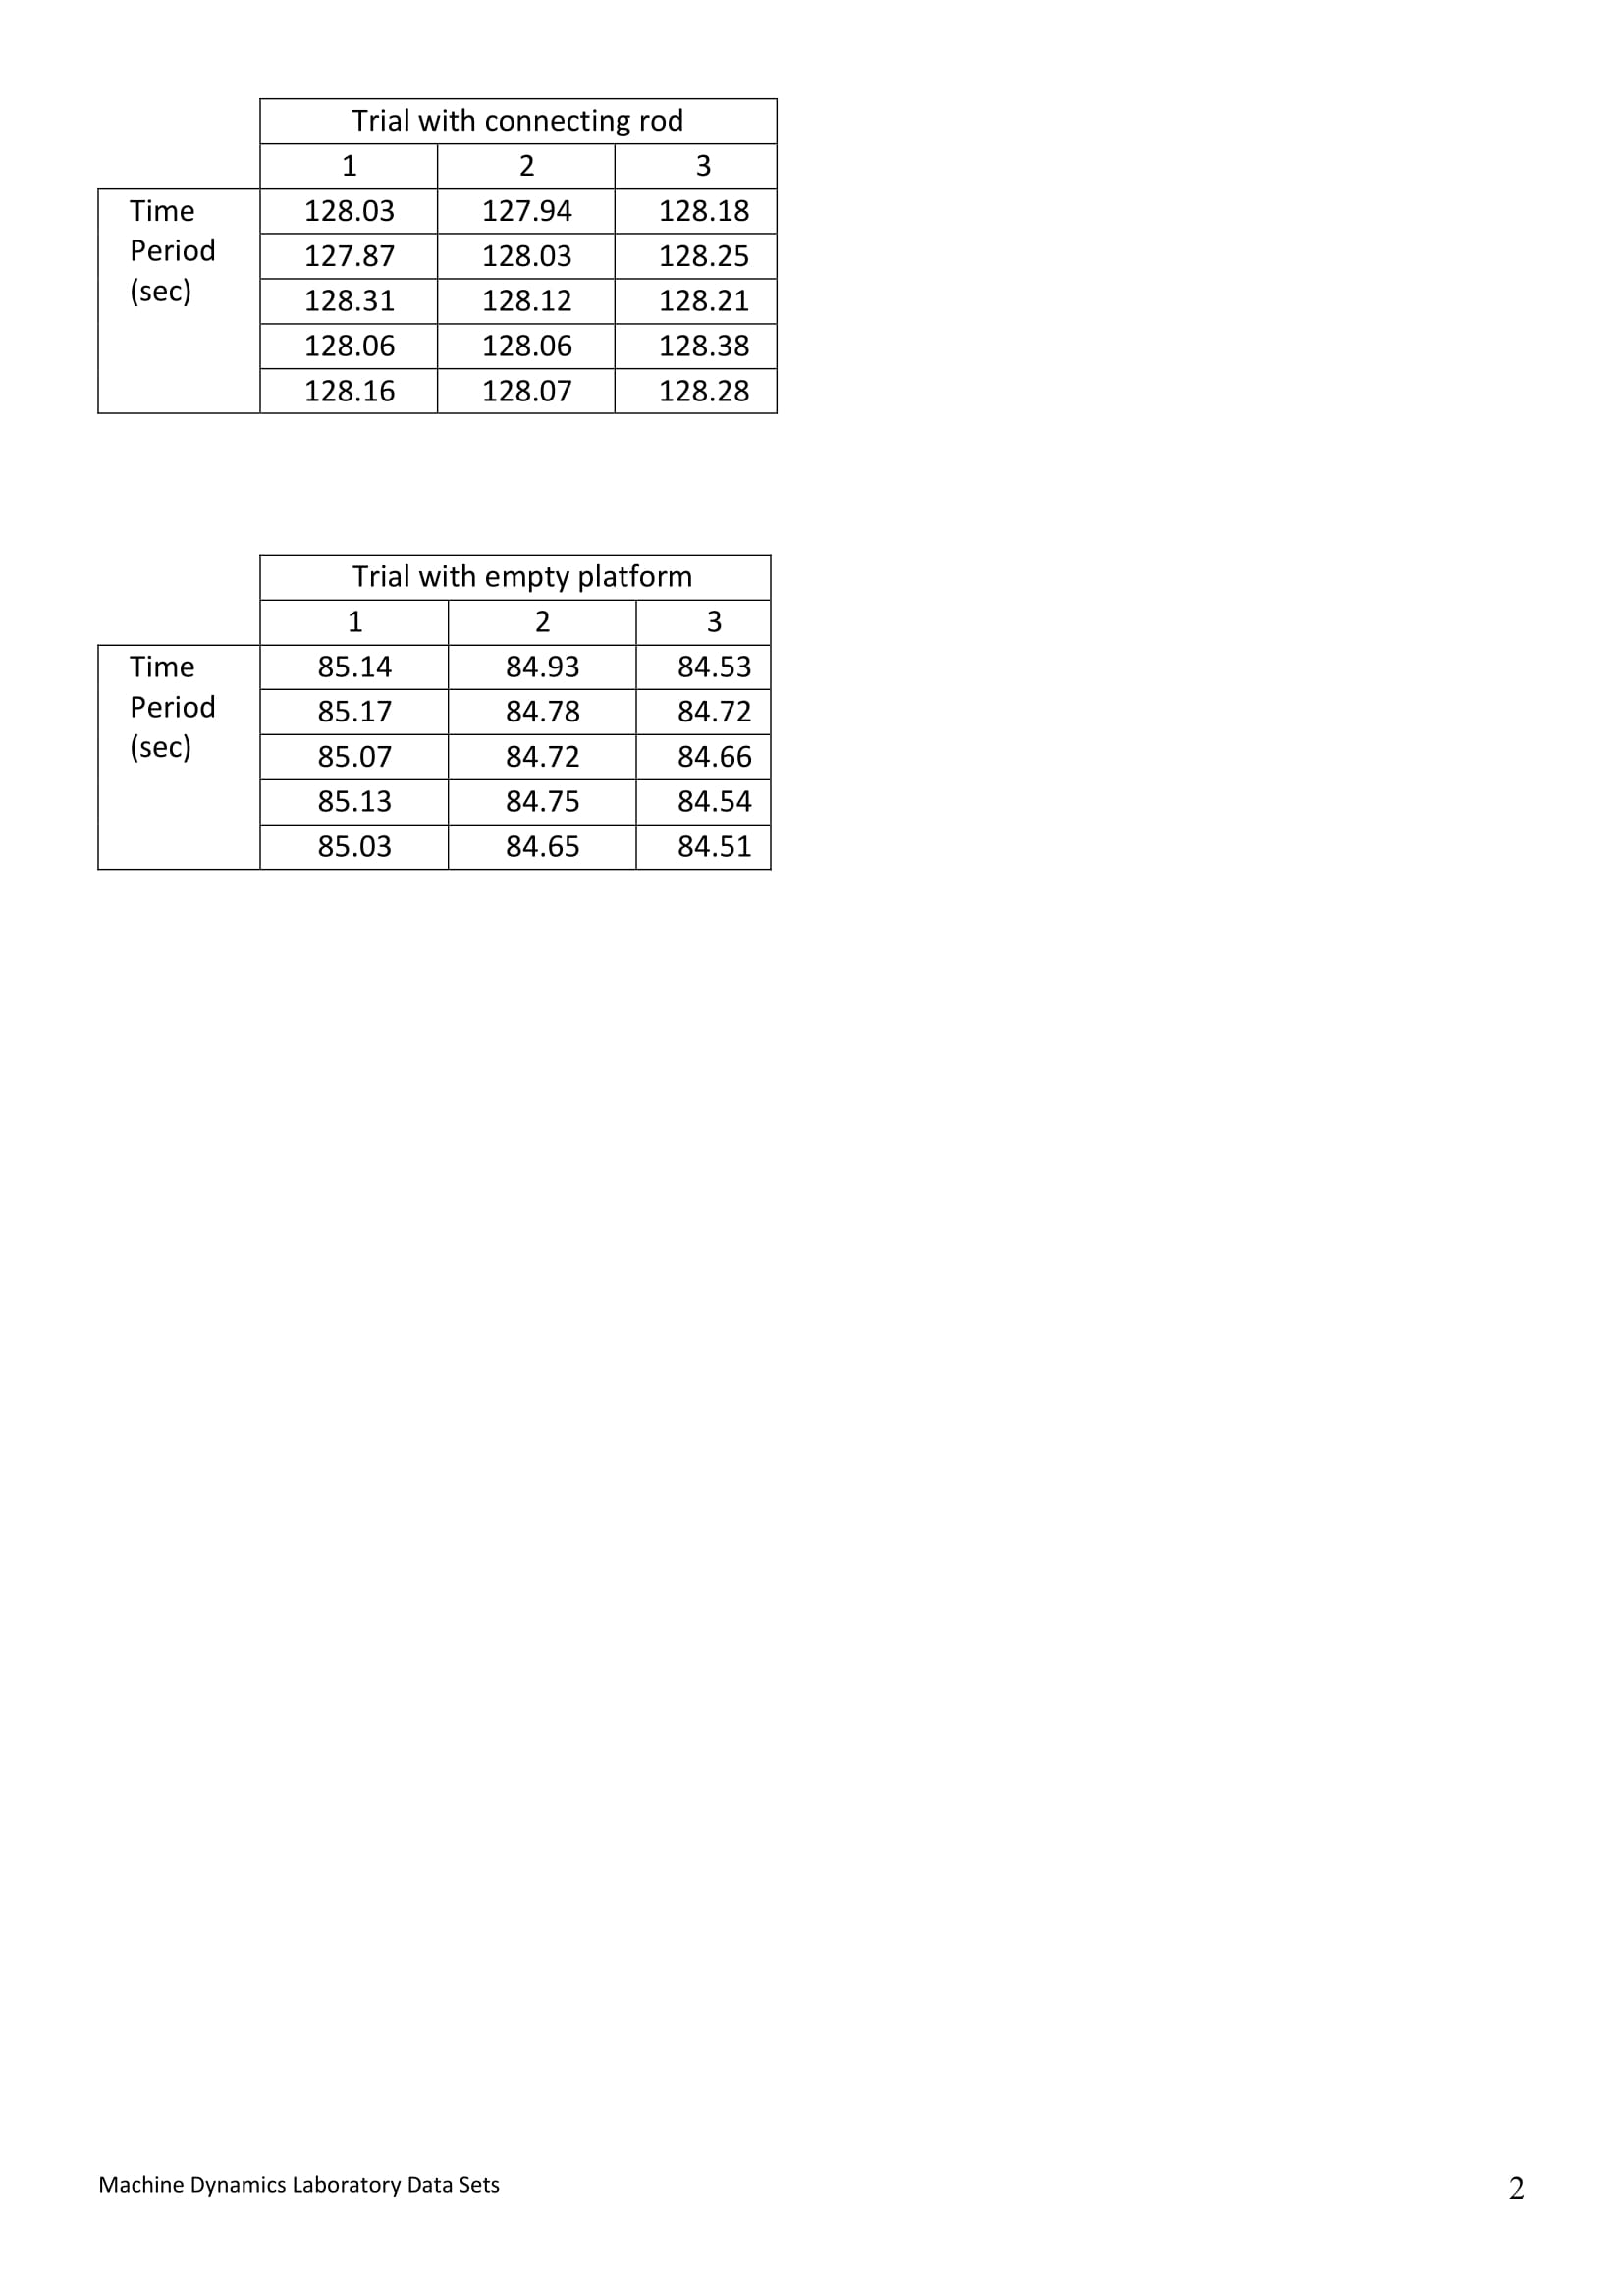
\includegraphics[width=\linewidth]{dataset/mass2}
  \caption*{}
\label{}
\end{figure}

\subsection*{7.3 Belt Friction Laboratory Script.}
\addcontentsline{toc}{section}{7.3 Belt Friction Laboratory Script.}
\begin{figure}[H]
  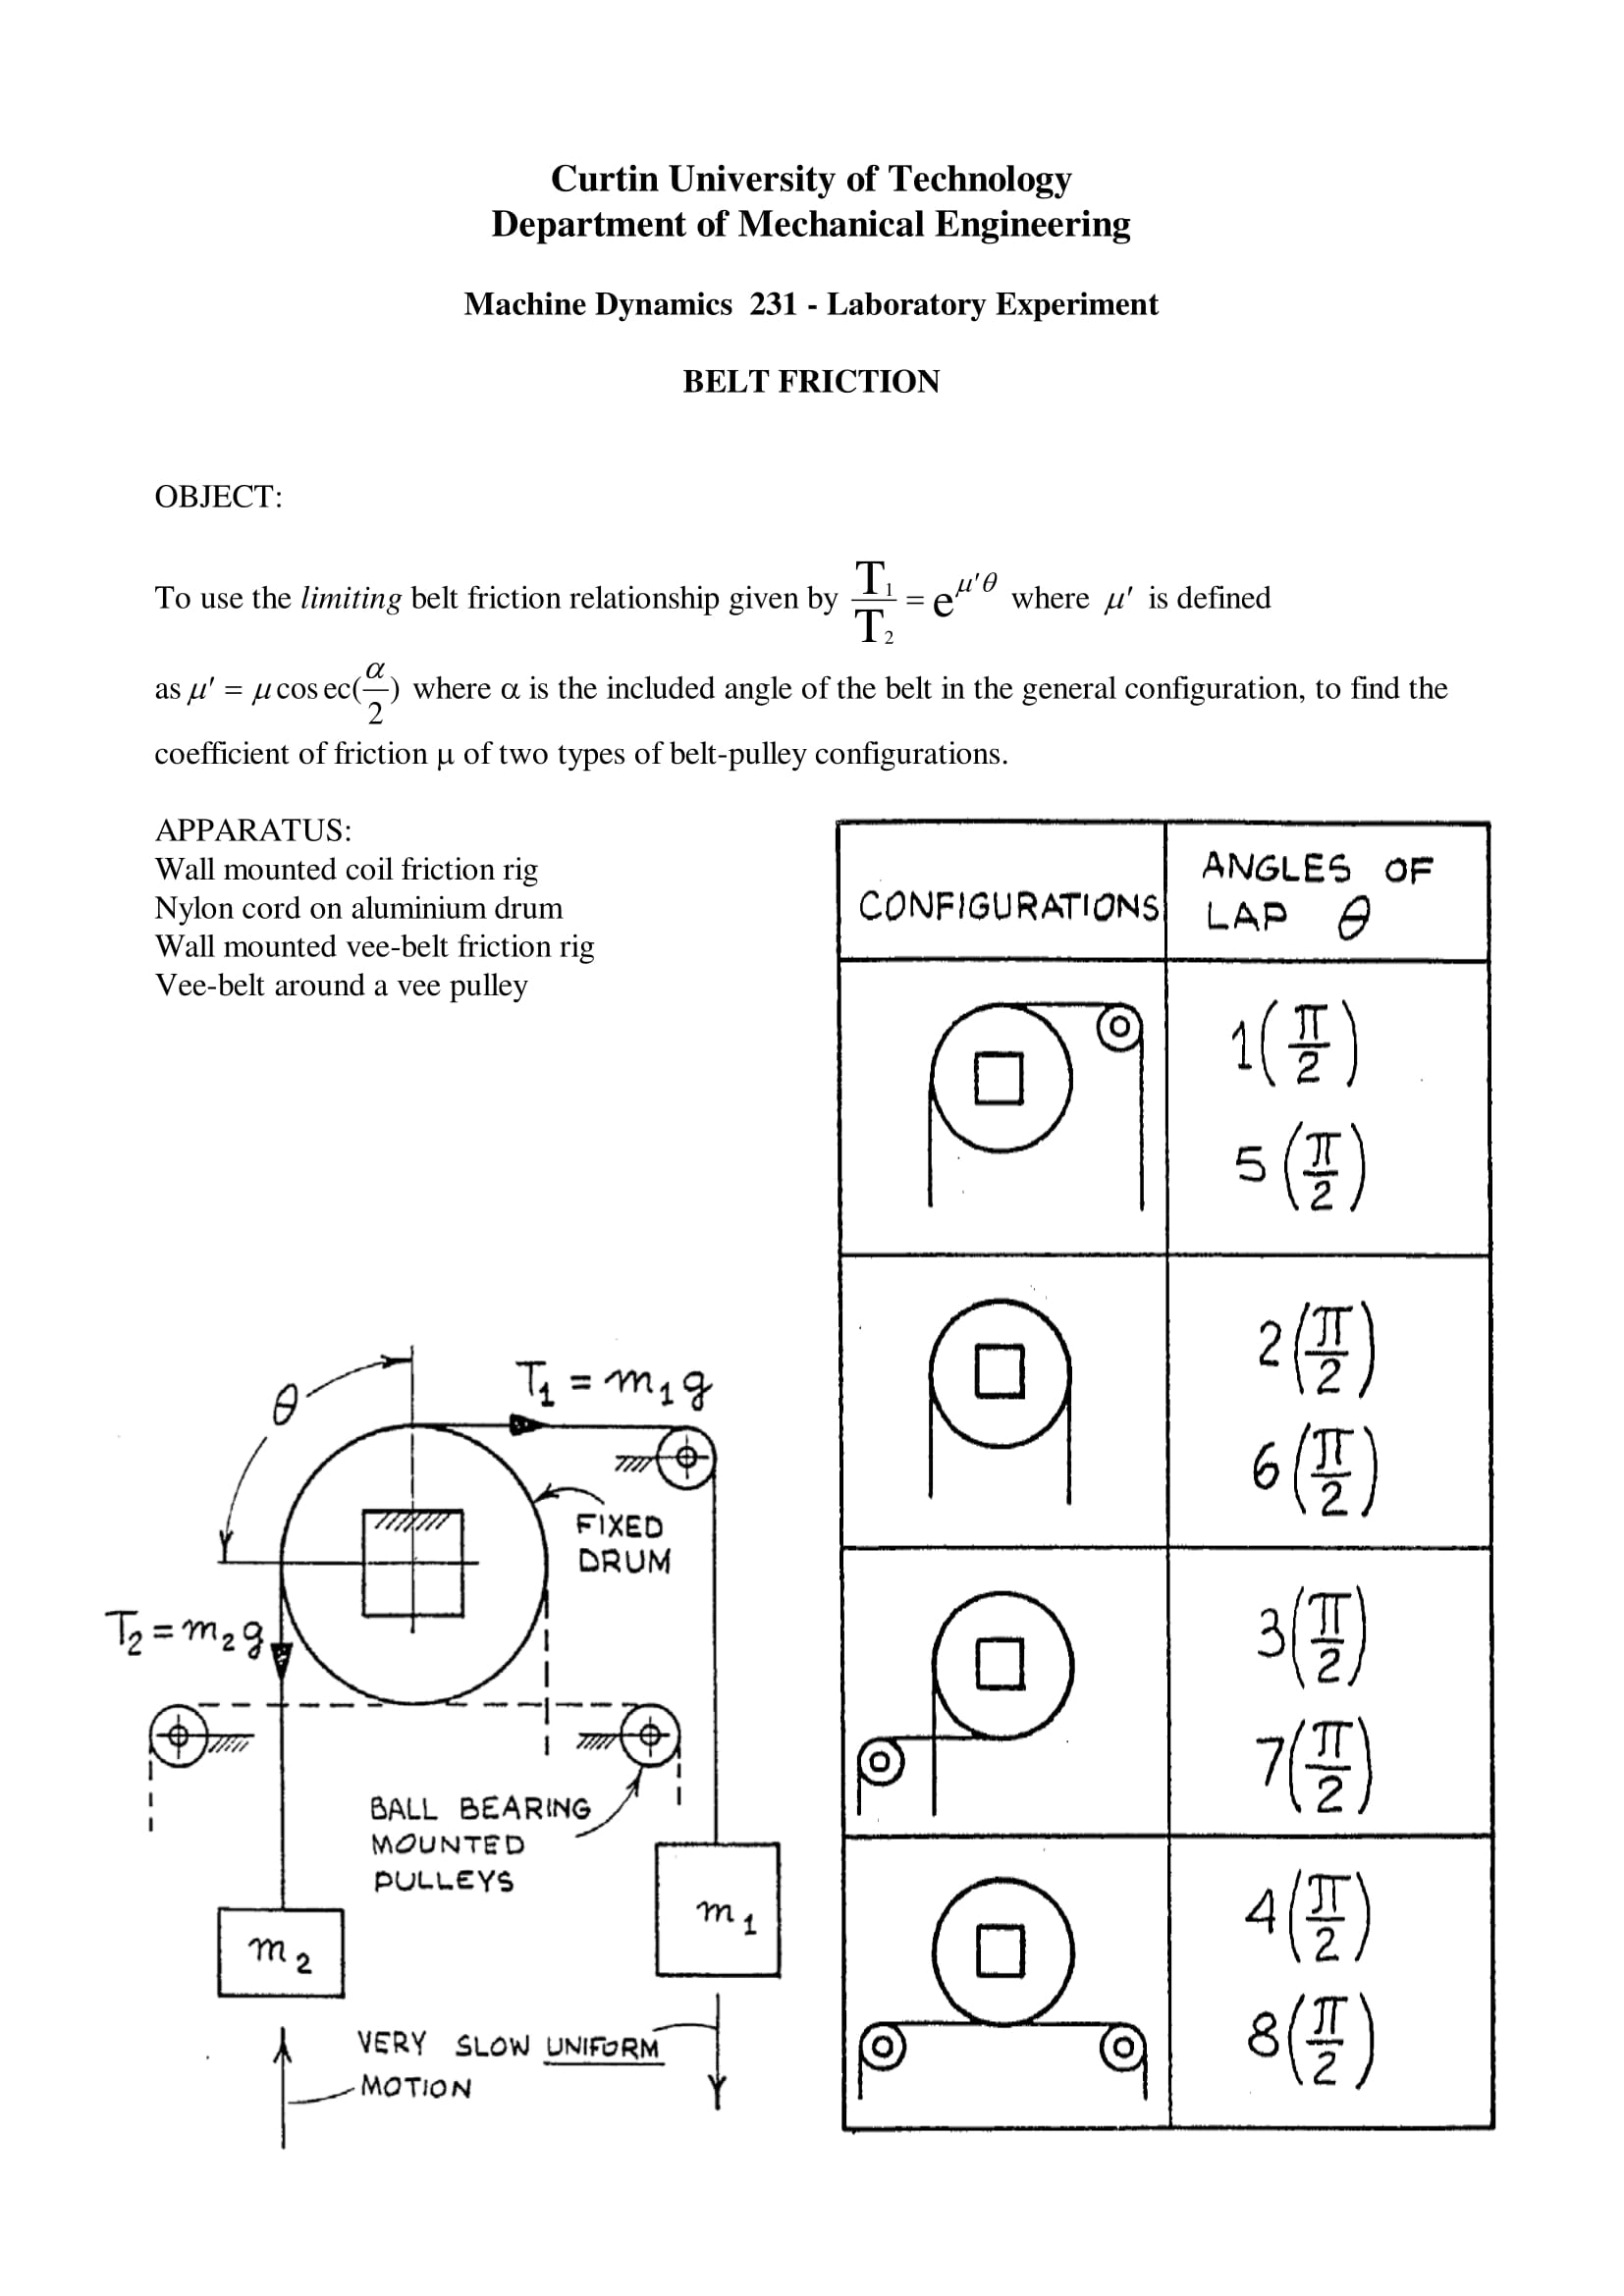
\includegraphics[width=\linewidth]{lab2/lab2-1}
  \caption*{}
\label{}
\end{figure}
\begin{figure}[H]
 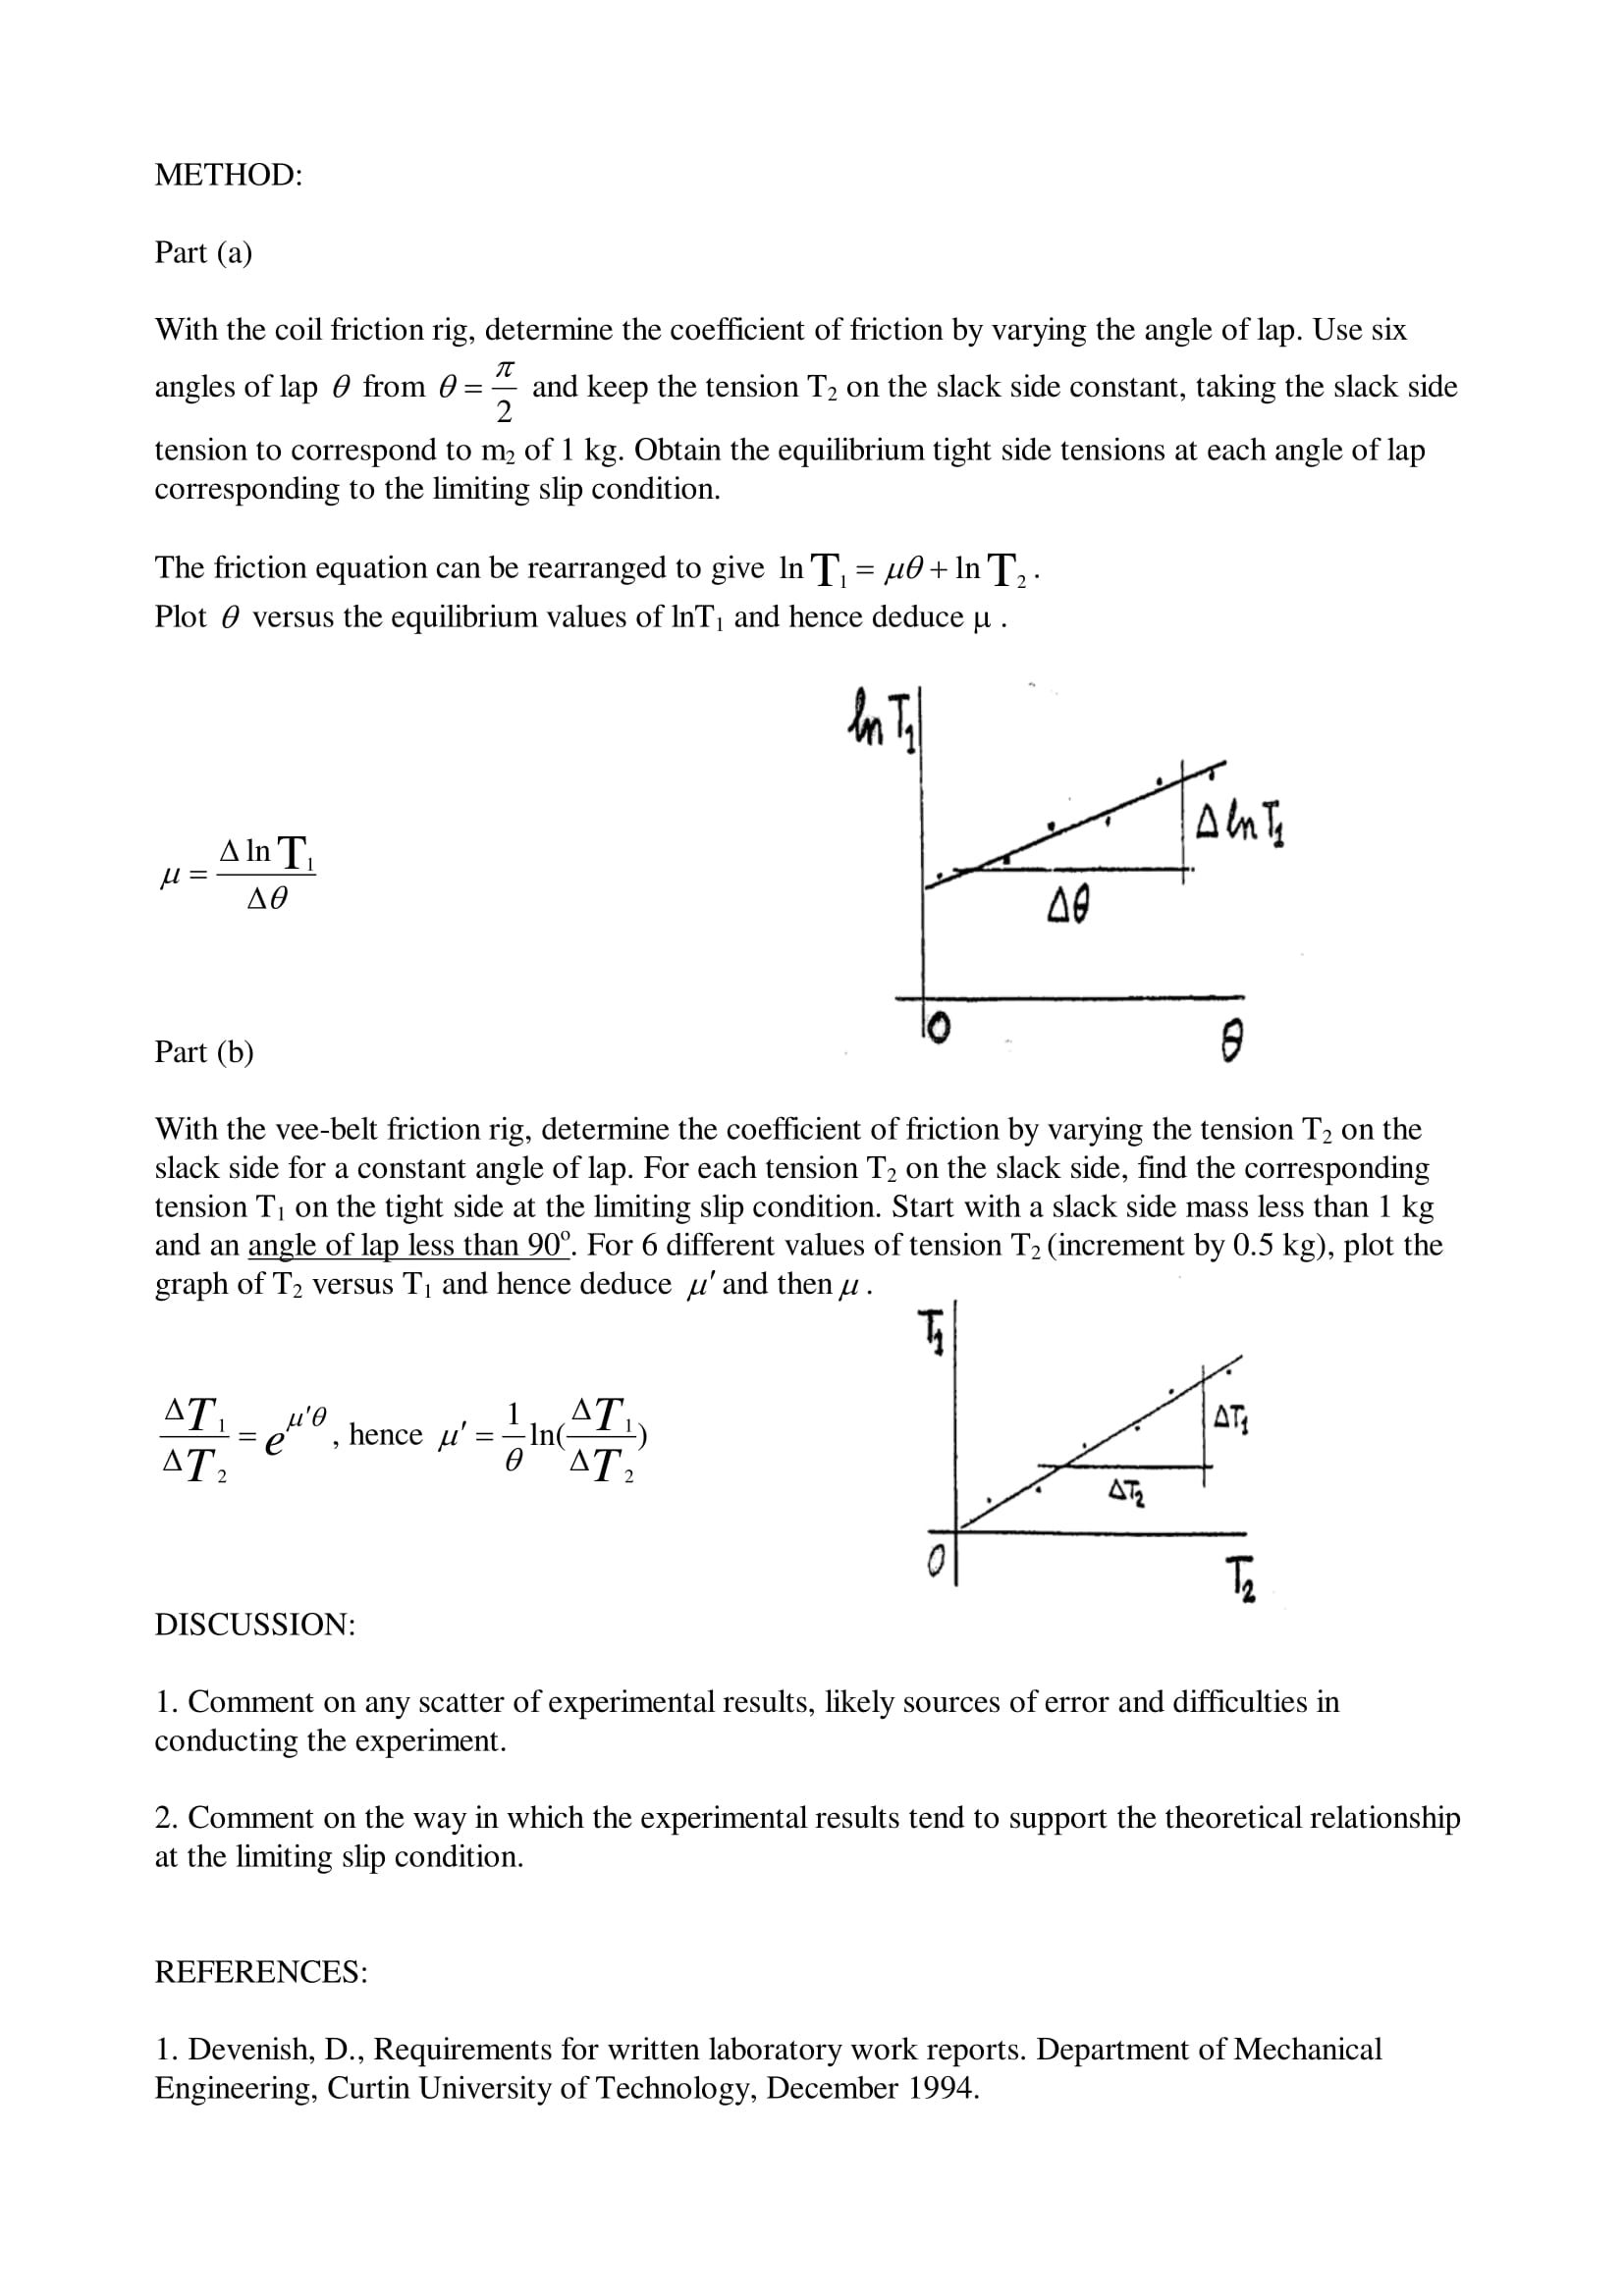
\includegraphics[width=\linewidth]{lab2/lab2-2}
  \caption*{}
\label{}
\end{figure}

\subsection*{7.4  Experimental Results for Belt Friction Experiment.}
\addcontentsline{toc}{section}{7.2  Experimental Results for Belt Friction Experiment.}
\begin{figure}[H]
  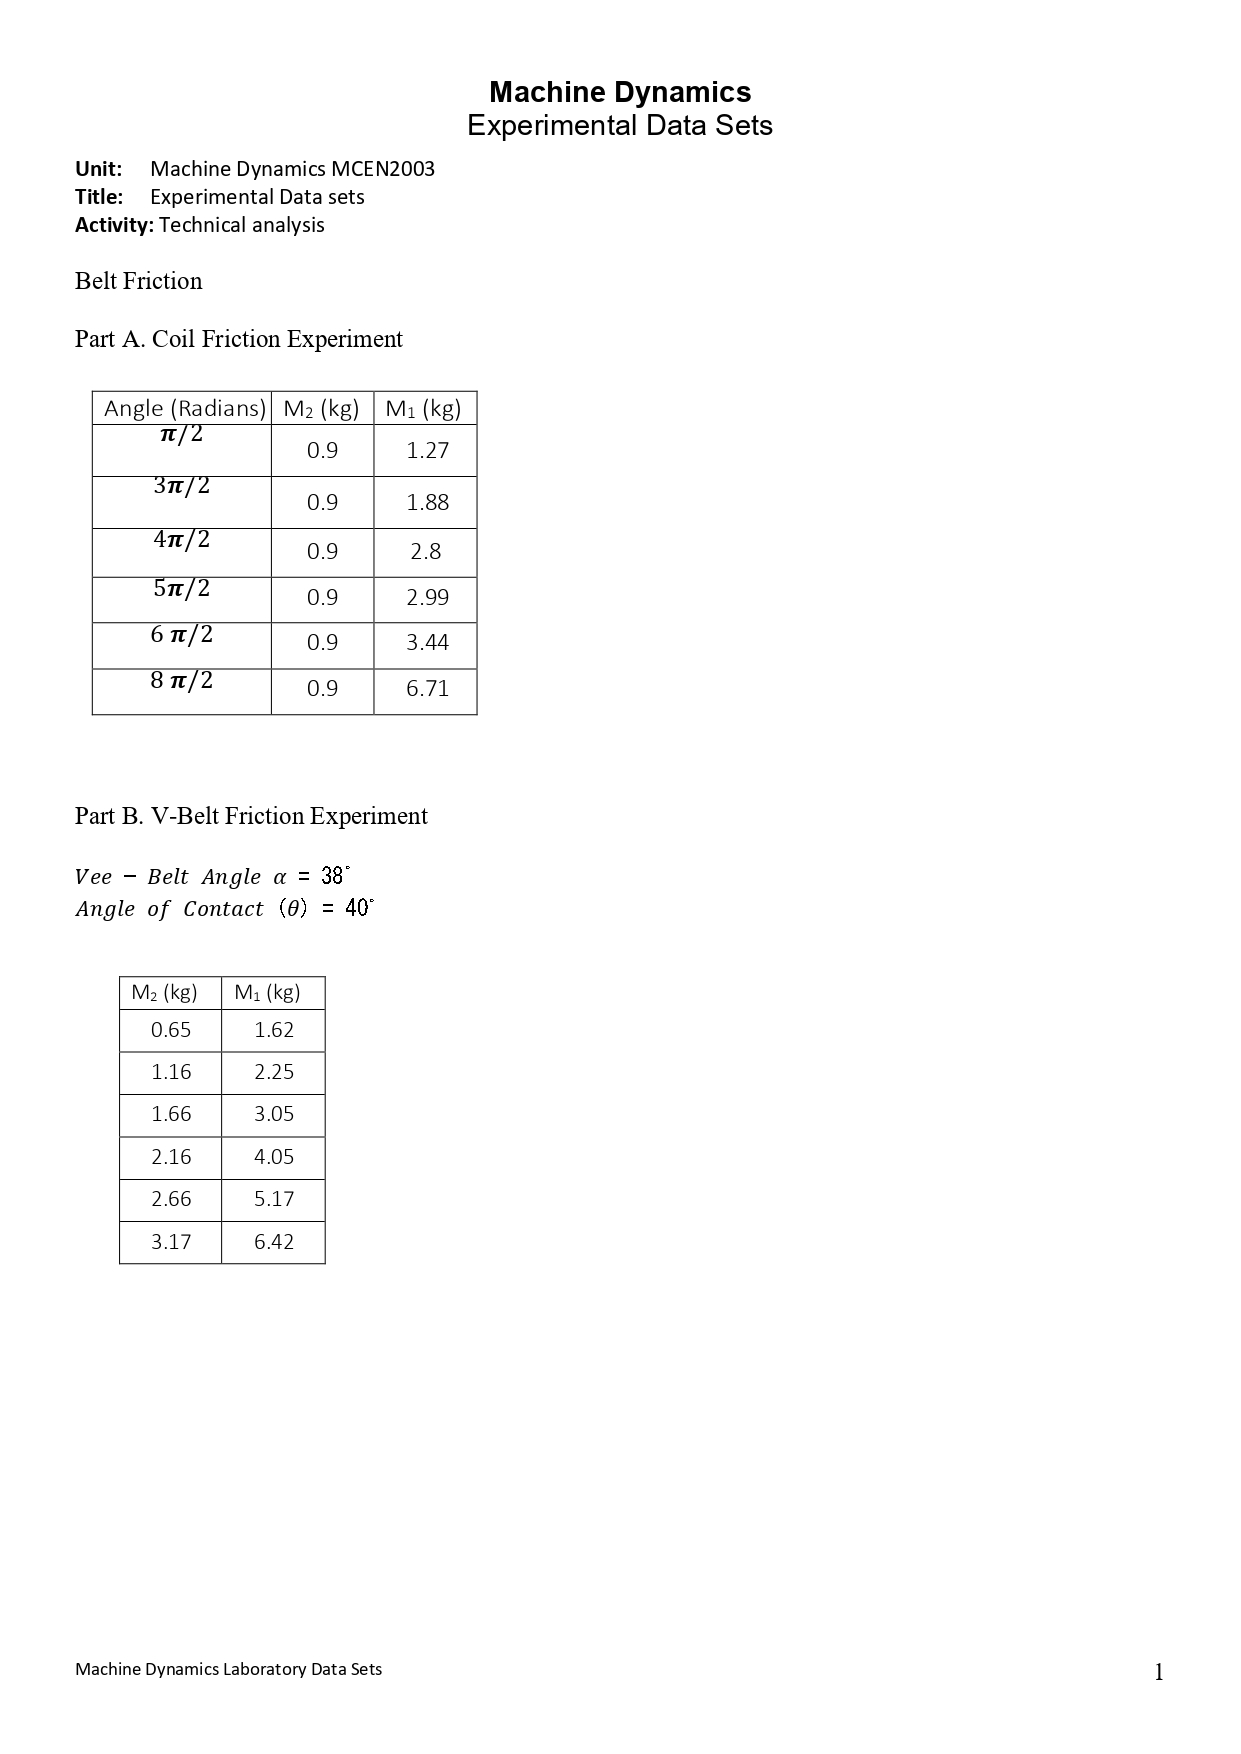
\includegraphics[width=\linewidth]{dataset/belt}
  \caption*{}
\label{}
\end{figure}

\subsection*{7.5 Epicylic Gears Laboratory Script.}
\addcontentsline{toc}{section}{7.5 Epicylic Gears Laboratory Script.}
\begin{figure}[H]
  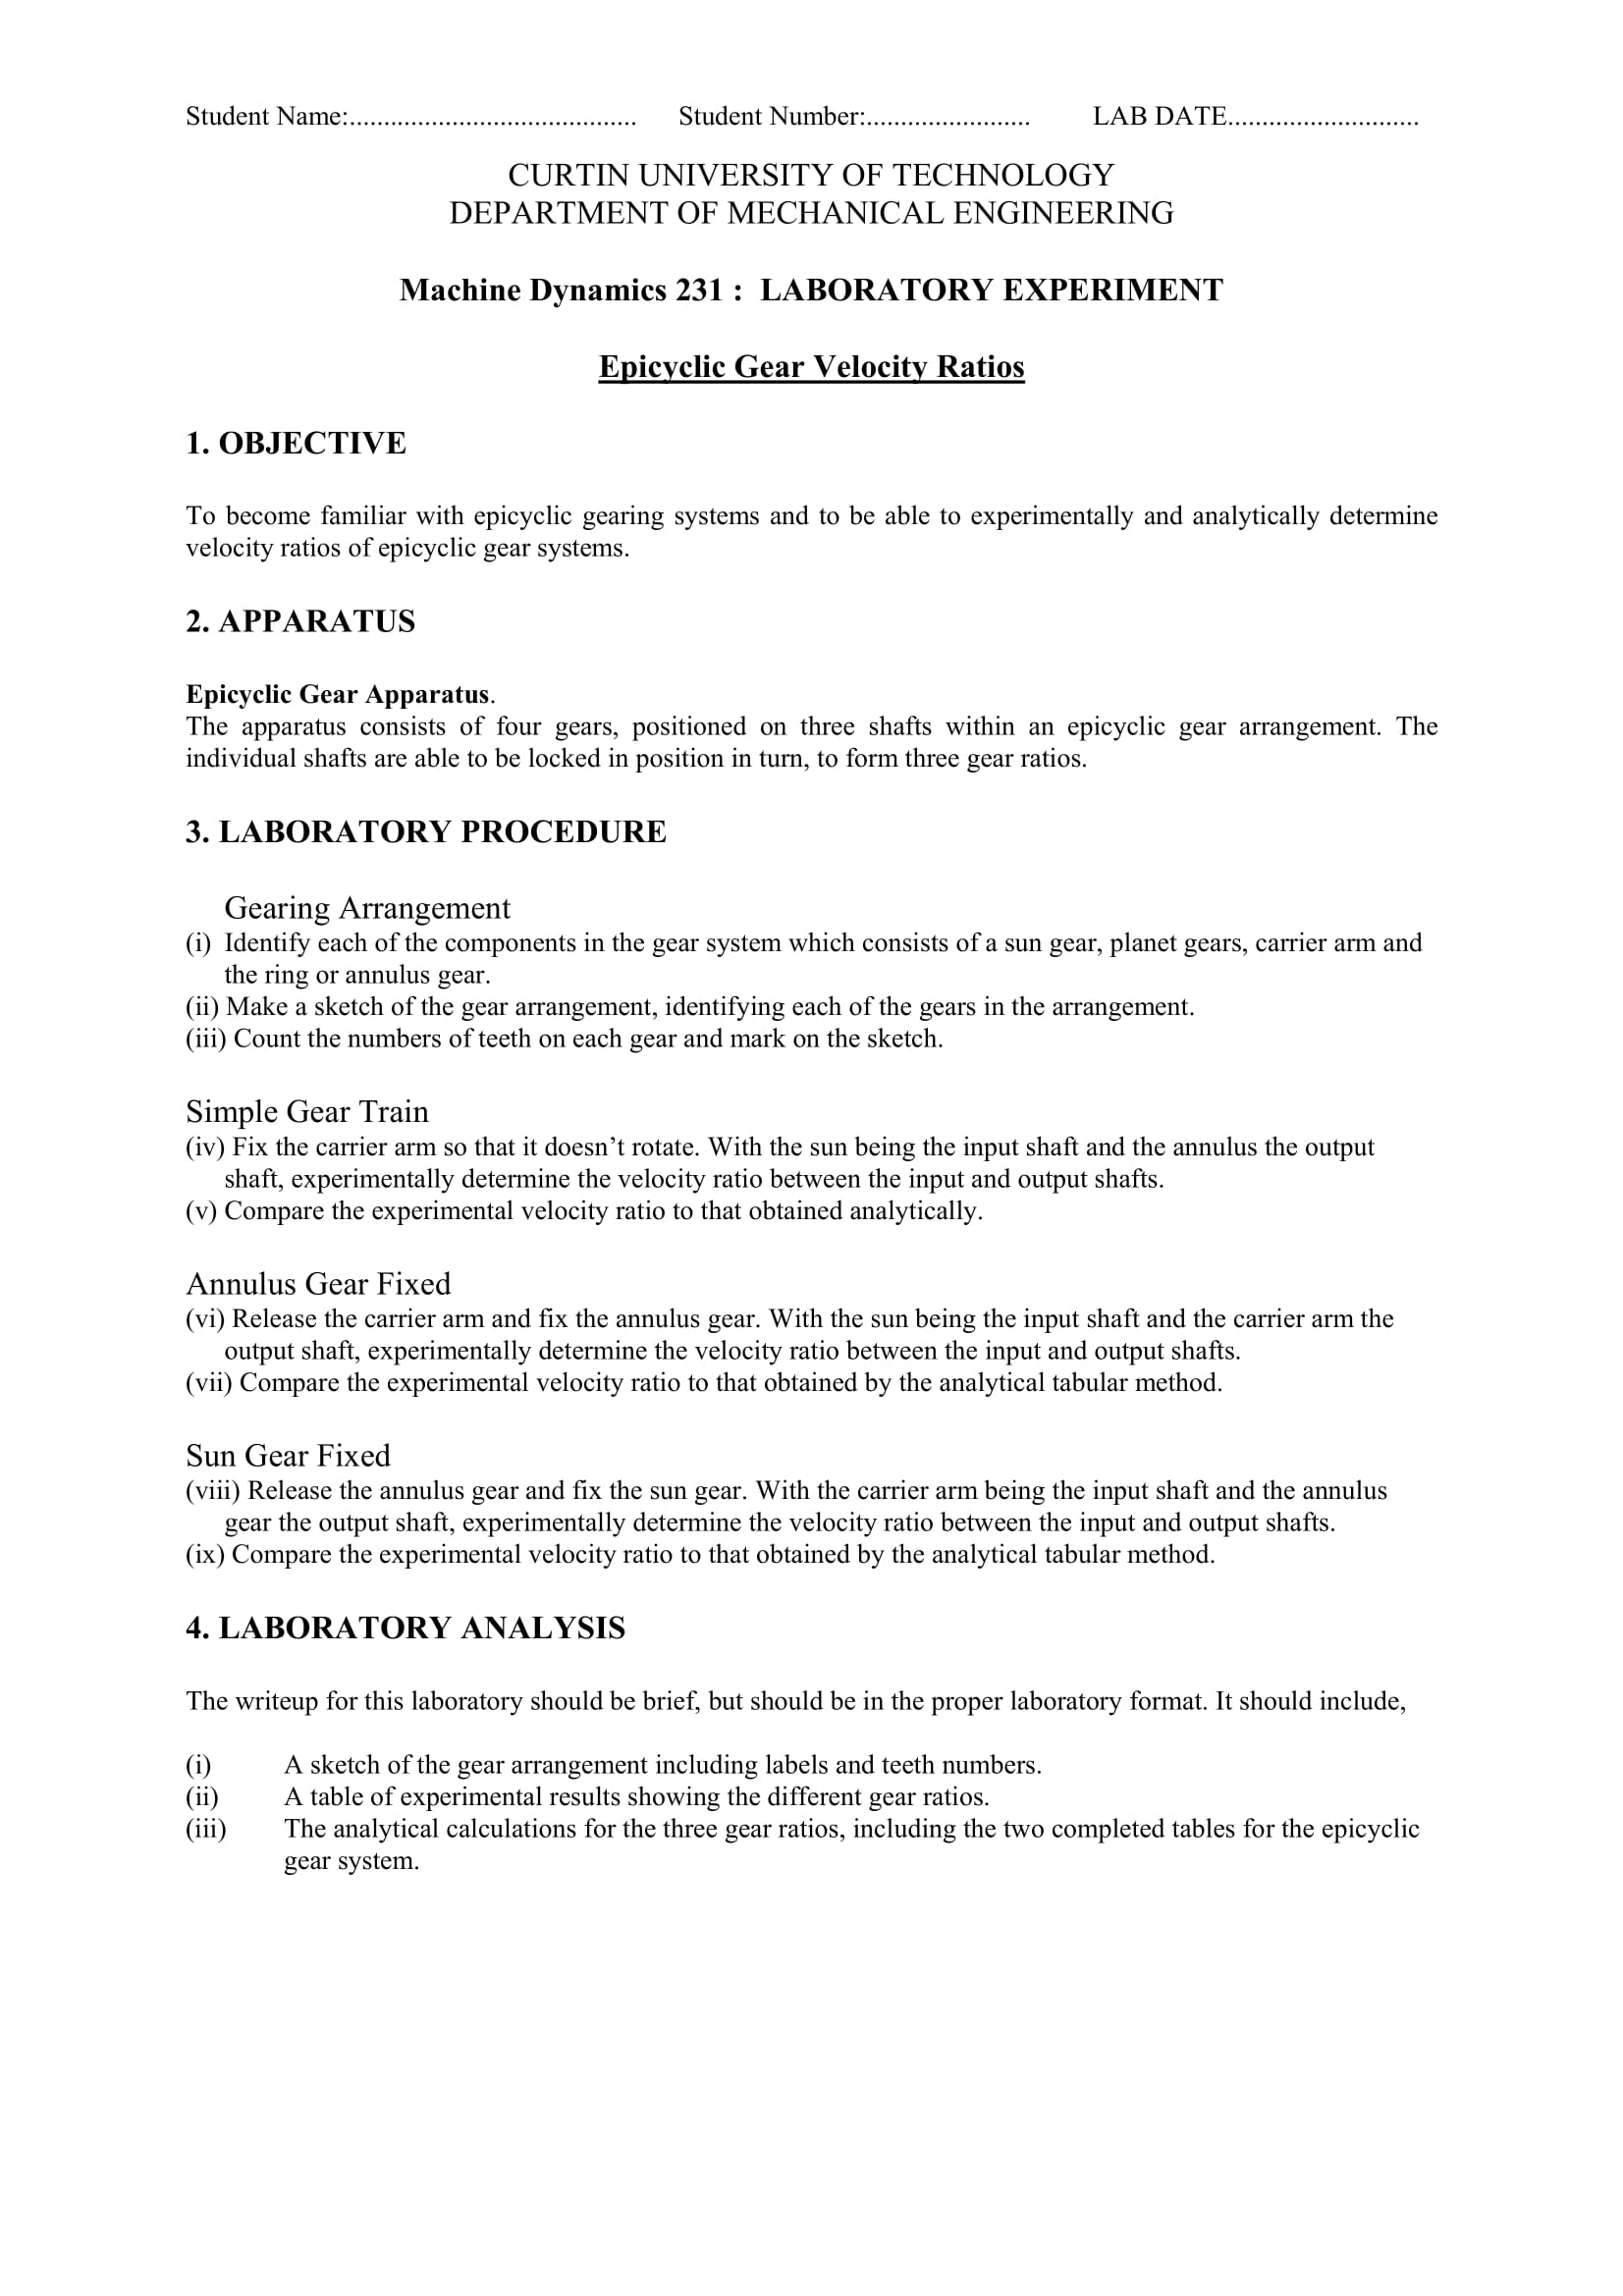
\includegraphics[width=\linewidth]{lab3/lab3-1}
  \caption*{}
\label{}
\end{figure}

\subsection*{7.6 Error Analysis.}
\addcontentsline{toc}{section}{7.6 Error Analysis.}
\begin{figure}[H]
  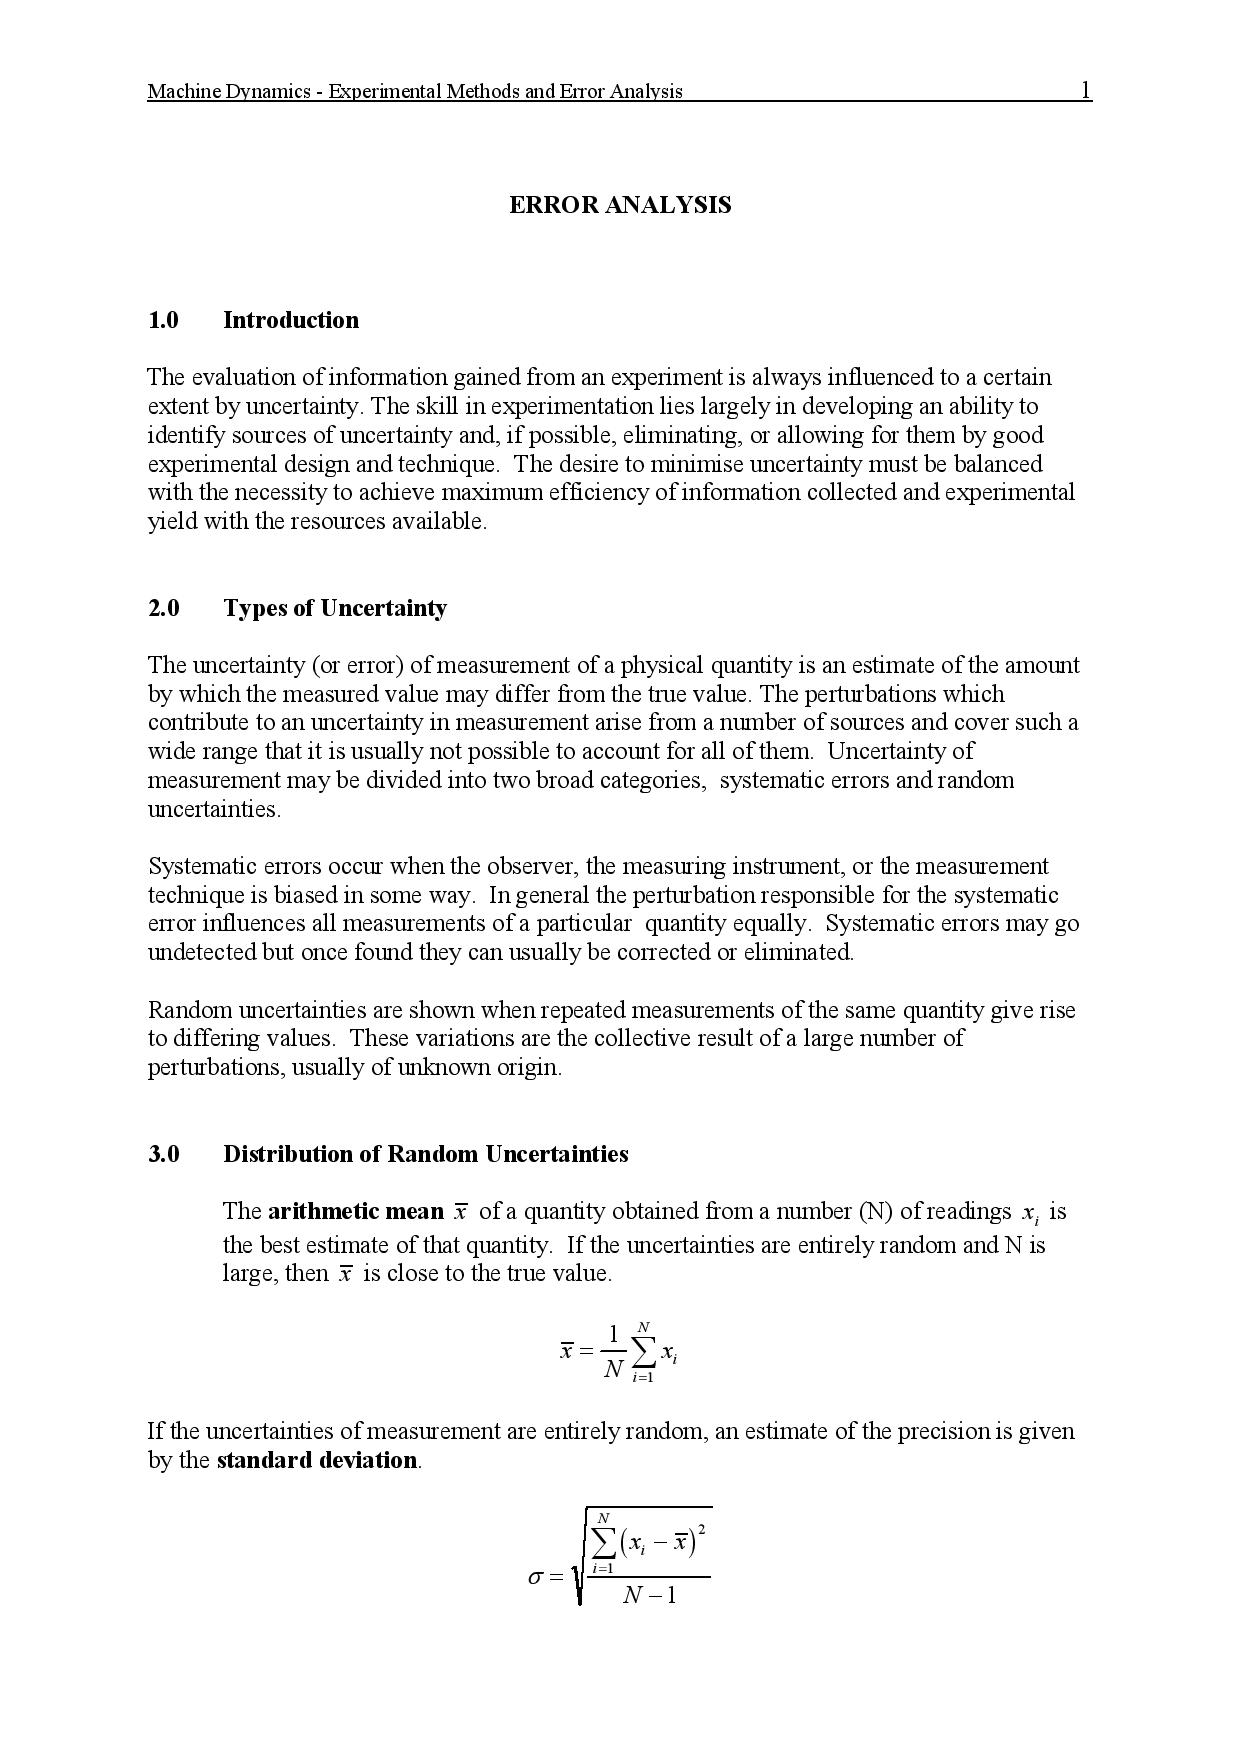
\includegraphics[width=\linewidth]{error/e1}
  \caption*{}
\label{}
\end{figure}
\begin{figure}
  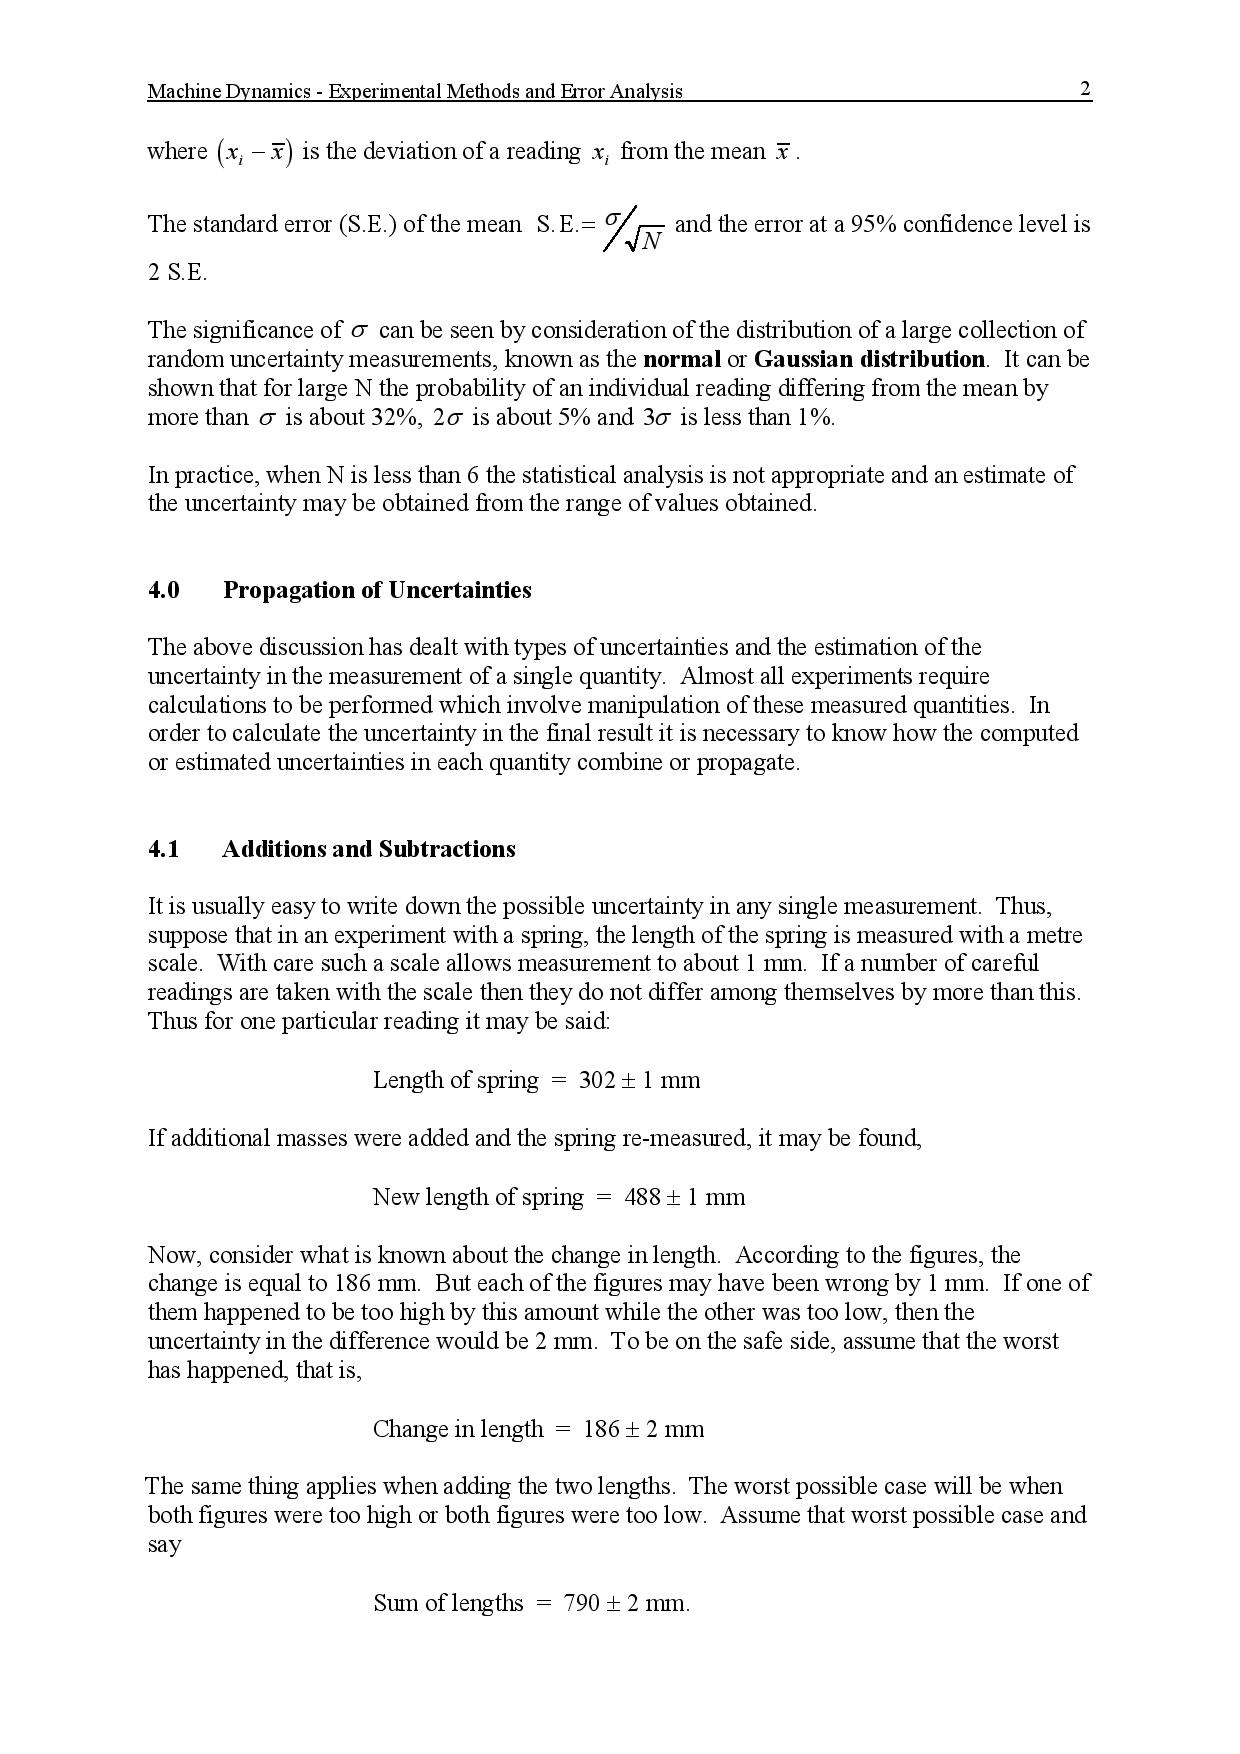
\includegraphics[width=\linewidth]{error/e2}
  \caption*{}
\label{}
\end{figure}
\begin{figure}
  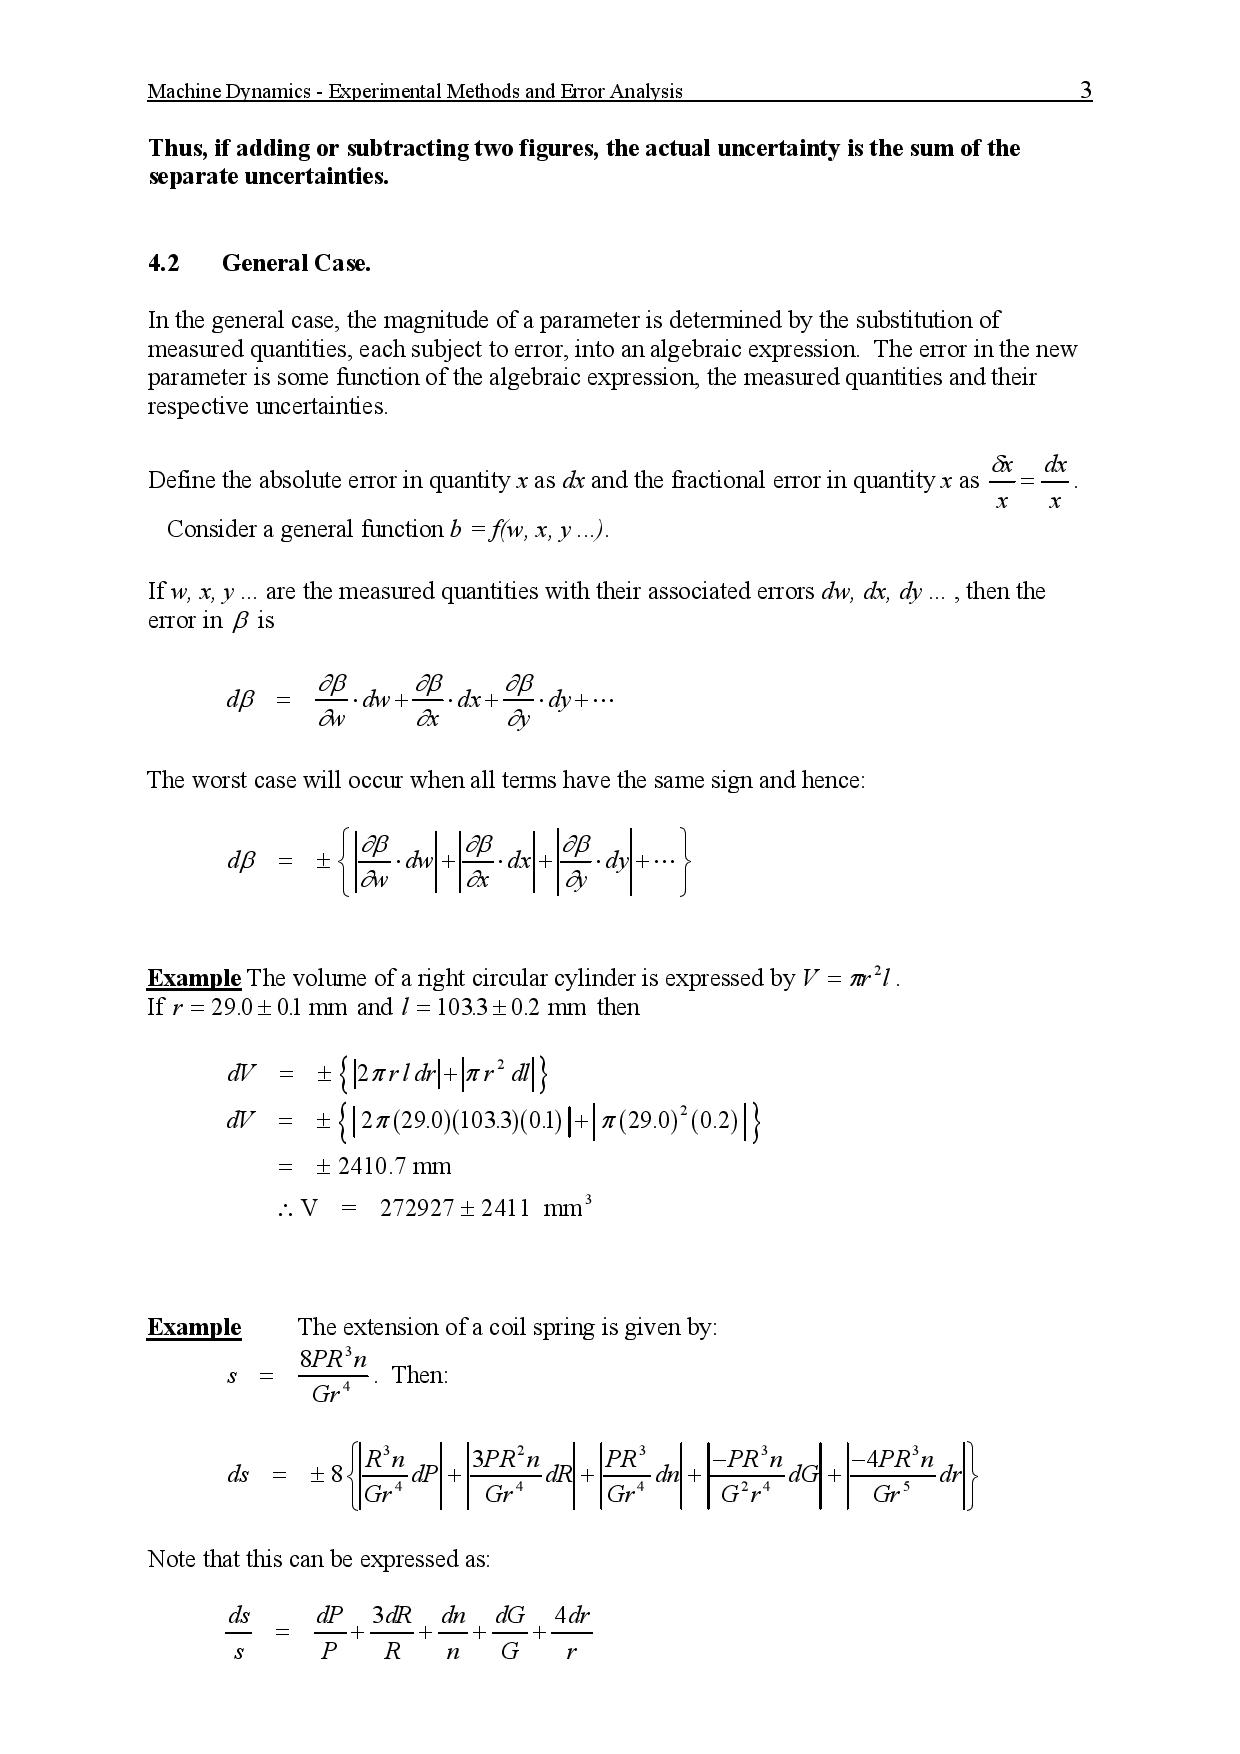
\includegraphics[width=\linewidth]{error/e3}
  \caption*{}
\label{}
\end{figure}
\begin{figure}
  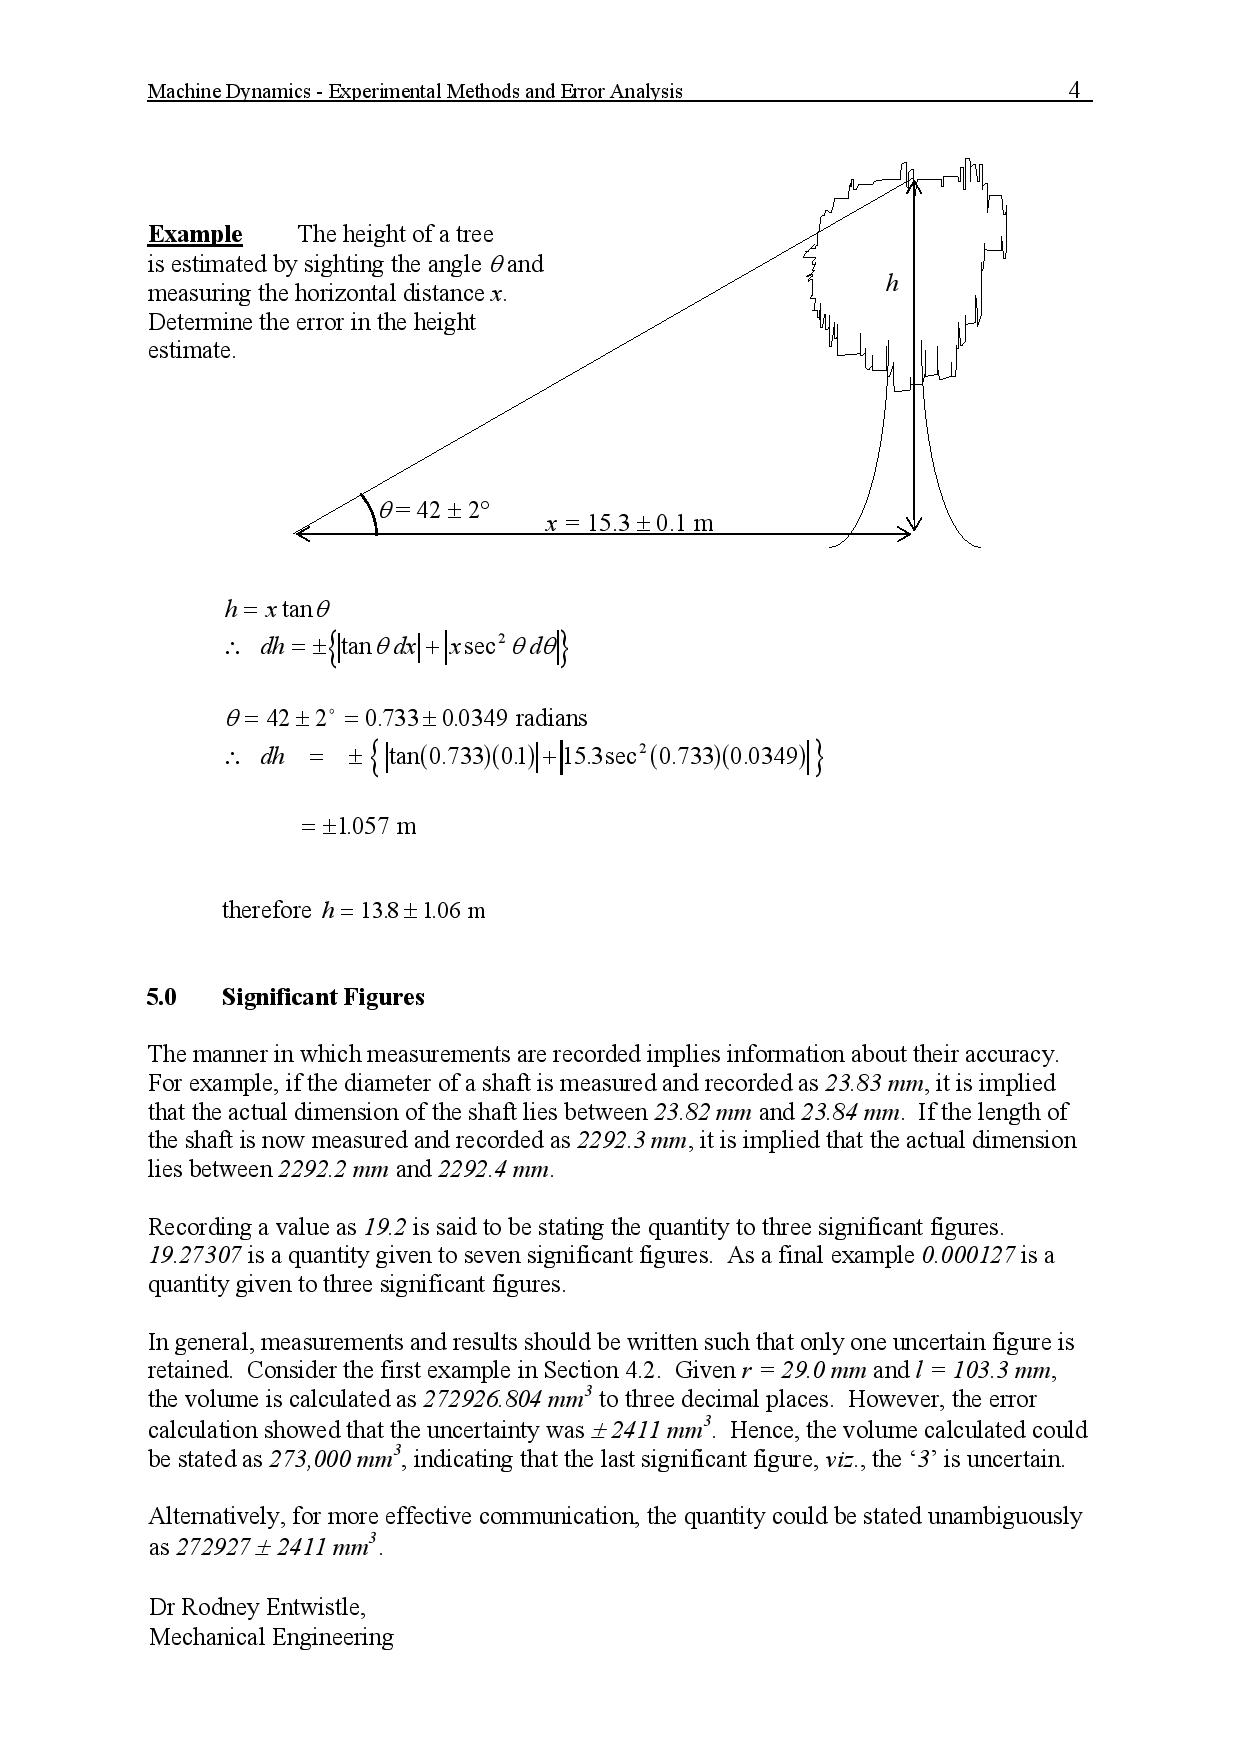
\includegraphics[width=\linewidth]{error/e4}
  \caption*{}
\label{}
\end{figure}

\end{document}